\chapter{Kochen-Specker contextuality}
\label{sec:kscontextuality}
\lhead{\emph{Kochen-Specker contextuality}}
Sections \ref{sec:threeboxes}-\ref{sec:bell} are in part adapted from.

The Kochen-Specker (KS) Theorem \cite{Kochen1968} is the often overlooked brother of Bell's monumental no-go theorem \cite{Bell1964}. In loose terms, Bell's Theorem proves that quantum mechanics (QM) cannot be described in terms of a local hidden variable model (HVM). A ``Bell inequality" is a condition measurement correlations must obey, for them to permit a local HVM description. Violations of Bell inequalities have been observed in numerous experiments: The well-known Delft experiment of 2015 was the first loophole-free confirmation of such violations \cite{Hensen2015}. As will be discussed in Section \ref{sec:bell}, Bell locality and KS non-contextuality are closely related, locality being the weaker assumption and justified by special relativity. Nevertheless, the KS Theorem has several distinct features that deserve to be studied in their own right. Most notably, KS contextuality allows one to examine how even single quantum systems are incompatible with a seemingly orthodox classical description in terms of hidden variables \cite{Pusey2019}. In contrast, Bell tests require two or more space-like separated quantum systems, in order for the measurement statistics to exhibit Bell non-locality. The reason for this is that we observe violations of Bell inequalities for entangled quantum systems. An immediate consequence is that the notion of KS contextuality applies to a much broader class of experiments.

\section[Introductory example\\ Specker's three boxes]{Introductory example\\ \large{Specker's three boxes}}
\label{sec:threeboxes}
Section \ref{sec:kscont} will give a formal definition of KS non-contextuality. Nevertheless, we shall first consider a simple example that illustrates the concept. It is taken from Specker's 1960 paper “The logic of propositions which are not simultaneously decidable” \cite{Specker1975}, which also gives a nice accompanying parable about an overprotective seer that teaches at the school of prophets in the fictitious place Arba’ila. Fairy tales aside, consider three boxes, labelled with 1, 2, 3, that can each be in one of two states: empty or containing a gem. The state of a box can be measured by opening the lid and peeking inside. Let $M_{1}$, $M_{2}$, $M_{3}$ denote the three two-outcome measurements (with outcomes “empty” or “gem”) of the boxes. Further assume, rather unnaturally, that it is impossible to open all three boxes simultaneously. Rather, only pairs of boxes may be jointly measured. Figure \ref{fig:3boxes} depicts the setting of Specker's “three boxes” example. For some repeatable preparation of the system, one curiously observes the following: opening pairs of boxes always yields anti-correlated measurement outcomes (that is, one of the boxes will be empty and the other will contain a gem). How can these statistics be reconciled with a naive model of reality that assumes the three boxes to be in some underlying state that specifies their contents? As we can only ever open two boxes simultaneously, we can never observe this hidden state of reality. Importantly, a valid assignment of gems to the three boxes must be compatible with the observed anti-correlated outcomes. It turns out, as the reader should convince themself, that any assignment of gems to the boxes is incompatible with the observed statistics. Assuming that the pairs of boxes to be measured are picked at random, in a uniform way, the probability of observing anti-correlated outcomes is bounded by $p(\text{anti-correlated})\leqslant\frac{2}{3}$ and we conclude that the naive type of HVM we just considered is unable to account for the experimental data.

\begin{figure}
\centering
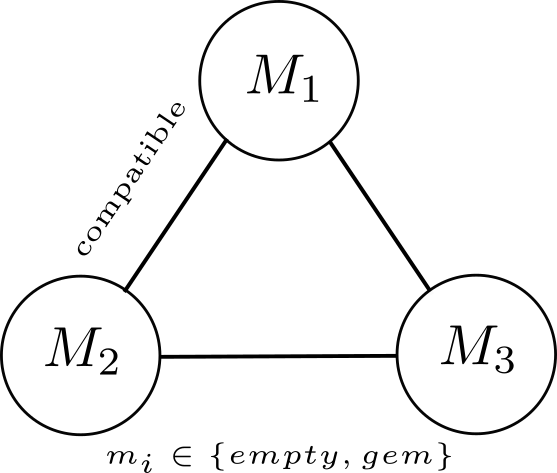
\includegraphics[width=0.4\textwidth]{images/3boxes.png}
\caption{Specker's ``three boxes" example. Three boxes 1,2,3 can each either hold a gem or be empty. The measurement $M_i$ corresponds to opening the lid of the $i$th box and checking its contents. The outcome of measurement $M_i$ is denoted by $m_i$. A solid line between measurements means that these are compatible and can be measured simultaneously. Despite all measurements being pairwise compatible, only pairs of boxes can be jointly measured. Measuring pairs of boxes always yields anti-correlated outcomes.}
\label{fig:3boxes}
\end{figure}

The point is that we have in fact considered a deterministic and non-contextual HVM to describe the three boxes. Deterministic just means that the underlying state of the system fixes all measurement outcomes and not just a probability distribution over possible outcomes. More interestingly, we define non-contextuality for the time being as the critical assumption that the outcome of some measurement should be the same, regardless of which other compatible\footnote{Two measurements are called \emph{compatible} if they can be performed simultaneously. While this ``definition" is sufficient for now, we will refine it in Section \ref{sec:correxp}.} measurement is performed simultaneously. Allowing the outcome of a measurement to depend on what other compatible measurement is performed together with it, could indeed account for the observed correlations.

\section{The Kochen-Specker Theorem, informally}
Informally, the KS Theorem states the following:

\begin{theorem}[Kochen-Specker, informal]
A non-contextual deterministic HVM of QM for Hilbert spaces of dimension $\geq3$ is impossible.
\end{theorem}

It is tempting to try to recast Specker's “three boxes” example to the realm of quantum theory. Within the theory of QM, compatible measurements are conventionally represented by commuting Hermitian operators. To implement the example in QM, we would have to find a quantum state $|\Psi\rangle$ and pairwise commuting two-outcome measurements $M_{1}$, $M_{2}$, $M_{3}$ not all simultaneously measurable, such that QM predicts $p(\text{anti-correlated})>\frac{2}{3}$. For the same reasons, this would imply that non-contextual deterministic HVM are not compatible with the predictions of QM and would prove the KS Theorem, albeit initially only for a fixed dimension that may be greater than 3. However, if all three measurements are pairwise commuting, they necessarily have a joint eigenbasis. Thus, all three measurements could be simultaneously performed and correlations with $p(\text{success})>\frac{2}{3}$ could not arise. Despite this, Sections \ref{sec:formalproof}, \ref{sec:4dim} feature examples that are similar in spirit, if a little more involved, and which can indeed be implemented by QM.

Specker hypothesized pairwise compatibility implying global compatibility to be the ``fundamental theorem of QM" that shapes the set of quantum correlations \cite{Cabello2012}. This is supported by the fact that for many correlation experiments the ``theorem" singles out correlations that are compatible with QM (and projective measurements) and offers an explanation for why quantum correlations cannot exceed certain mystifying bounds we will encounter in Section \ref{sec:cswhierarch} \cite{Cabello2013}.

Before we can discuss the KS Theorem and its proof in formal terms, as is done in Section \ref{sec:formalproof}, we will begin by establishing a general mathematical framework of HVM in Section \ref{sec:hvm}. Section \ref{sec:mnts} introduces two ways of representing measurements in QM, leading to two equivalent notions of KS non-contextuality, as defined in Section \ref{sec:kscont}. Section \ref{sec:4dim} presents a considerably simpler proof of the KS Theorem that holds for four-dimensional systems. The connection between KS non-contextuality and local causality will be the subject of Section \ref{sec:bell}, highlighting the similarities and differences between the KS Theorem and Bell's Theorem. This discussion will point out several flaws of the traditional notion of KS contextuality and addresses the need for an operational notion. A proposal of that sort by Spekkens will be introduced later in Section \ref{sec:spekkcont}. Finally, in Section \ref{sec:kcbs} we will discuss an important class of KS contextuality experiments involving a qutrit, namely the KCBS scenario and generalizations of it. For these experiments one can derive KS non-contextuality inequalities on the convex set of possible correlations, analogously to Bell inequalities, that must hold for all non-contextual statistics. Interestingly, these inequalities turn out to be incompatible with the predictions of QM for some quantum states.

\section{General framework of hidden variable models}
\label{sec:hvm}
An ontological model of QM\footnote{The following applies more generally for ontological models of arbitrary operational theories. An operational theory is one that makes testable predictions.}, more commonly referred to as a hidden variable model (HVM), presupposes some ontic state space $\Lambda$. An ontic state $\lambda\in\Lambda$ is a state of reality or “matter of fact” description of the system. It holds all attributes of the system, regardless of whether they are known or even knowable (hence hidden variables). Importantly, a HVM posits that our system is at each time point in some ontic state with corresponding definite attributes, even when these are not being subjected to measurements. In the case of KS contextuality we will only consider \textbf{deterministic} HVM, meaning that an ontic state fixes the outcomes of all possible measurements that may be performed on the system. Uncertainty in the ontic state that was prepared results in a probabilistic distribution of measurement outcomes. It is helpful to formalize this and boil the assumptions down to a simple mathematical model. We follow the notation and terminology of \cite{Spekkens2005}.

With any preparations $P$ one can associate a probability density function $\mu_{P}(\lambda)$ on the ontic state space $\Lambda$. One can think of a preparation as an ensemble of systems, much like in the spirit of statistical mechanics, whereby each individual member of the ensemble is in some well-defined ontic state $\lambda\in\Lambda$. The probability of picking a system from the ensemble at random with a hidden parameter contained in some region $\mathcal{A}\subset\Lambda$, is then given by $\int_{\mathcal{A}}\mu_{P}(\lambda)d\lambda$. By normalization, we require that $\int_{\Lambda}\mu_{P}(\lambda)d\lambda=1$.

Measurements $M$ can be associated with sets of indicator functions $\left\{ \xi_{M,k}\right\} _{k}$ on $\Lambda$, one for each measurement outcome $k$. The value $\xi_{M,k}(\lambda)\in\{0,1\}$ is the conditional probability of the measurement $M$ yielding the outcome $k$, given that the system is in the ontic state $\lambda$. Since we are considering only deterministic HVM, meaning that the ontic state of the system fixes all measurement outcomes with certainty, this conditional probability must be either 0 or 1. Naturally, the indicator functions for the different measurement outcomes must obey $\sum_{k}\xi_{M,k}(\lambda)=1$ $\forall\lambda\in\Lambda$. Section \ref{sec:mnts} will introduce two ways of representing measurements in QM. We will apply the framework introduced in this section to these, in order to treat quantum measurements within HVM. Lastly, for the HVM to be consistent with the testable predictions of the operational theory it should model, it must hold that: $p(k\vert P,M)=\int_{\Lambda}d\lambda\thinspace\xi_{M,k}(\lambda)\mu_{P}(\lambda)$, where $p(k\vert P,M)$ describes the probability of observing the measurement outcome $k$, given measurement $M$ and preparation $P$, as predicted by the operational theory. The above quantities are pictorally summarized in Figure \ref{fig:hvm}, for the case of a two-outcome measurement $M$. In the following, when making reference to an arbitrary deterministic HVM of QM, we will implicitly assume an underlying ontic state space $\Lambda$ and indicator functions $\{\xi_{M,k}\}_{k}$ for all measurements $M$ with possible outcomes $k$.

\begin{figure}
    \centering
    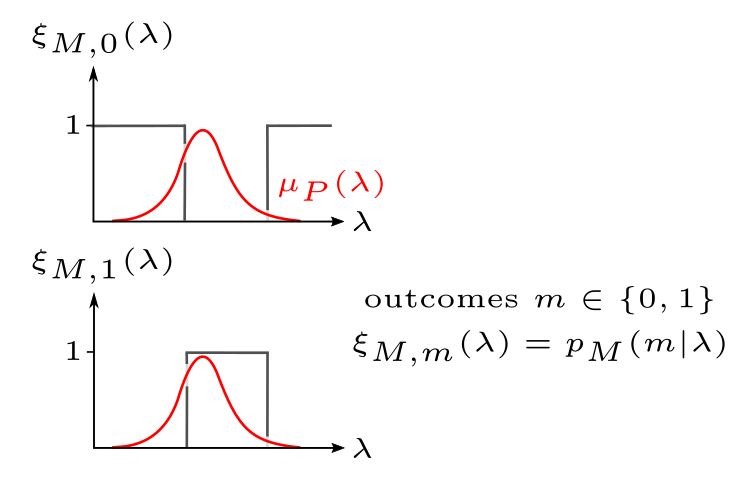
\includegraphics[width=0.7\textwidth]{images/hvm.png}
    \caption{Summary of the constituents characterizing a deterministic HVM for the case of a two-outcome measurement.\hfill\break A system's ontic state space $\Lambda$, here depicted as a one-dimensional axis, comprises all possible states of reality. A state preparation $P$ can be associated with a probability density function on $\Lambda$, modelling the uncertainty in the prepared ontic state. A deterministic HVM associates with any measurement $M$, here a two-outcome measurement with outcomes $m\in\{0,1\}$, a set of indicator functions $\{\xi_{M,m}\}_m$. The indicator function to measurement outcome $m$, $\xi_{M,m}:\Lambda\rightarrow\{0,1\}$, maps each ontic state to the probability of observing outcome $m$, conditioned on the system being in that ontic state.}
    \label{fig:hvm}
\end{figure}

\section{Measurements in quantum mechanics}
\label{sec:mnts}
Section \ref{sec:kscont} will define the notion of KS non-contextuality that is at the heart of the KS Theorem. It is an assumption about the type of HVM the theorem rules out and, in loose terms, pertains to the measurements within such a HVM. To set the stage for discussing KS non-contextuality, this section introduces two ways of representing (projective) measurements in QM. As will be proved in Section \ref{sec:kscont}, the two notions of measurements will give us two equivalent notions of KS non-contextuality, each of which will be particularly useful for certain purposes. Note that within the framework of KS contextuality we assume all quantum measurements to be projective. On the other hand, in quantum information theory, a general quantum measurement is given by a set of positive semi-definite operators that sum to the identity, a so-called positive operator valued measure (POVM) \cite{Nielsen2010}. A projective measurement, or projection-valued measure (PVM), is also a POVM, however the reverse generally does not hold. The two are related in the sense that every POVM can be seen as a PVM acting on an extended Hilbert space, followed by us discarding some degrees of freedom, a consequence of Naimark's dilation theorem \cite{Watrous2018}. Thus, assuming all quantum measurements to be projective is in principle consistent with the existence of POVMs. In Section \ref{sec:spekkcont}, we present a revision of the traditional notion of KS contextuality due to Spekkens. Spekkens contextuality is defined largely in terms of operational primitives and is able to accommodate more general POVM quantum measurements. As physical measurements are non-ideal, we must account for these in view of our goal to certify quantum properties of a single quantum device under operational assumptions.

The conventional way of representing projective measurements in QM is in terms of Hermitian operators, with every measurement being relatable to a set of pairwise commuting and thus simultaneously measurable operators that share a common eigenbasis. Measurement outcomes are tuples of simultaneous eigenvalues. The spectrum of a Hermitian operator A is denoted by $\sigma(A)$ and the set of all Hermitian operators on a Hilbert space $\mathcal{H}$ is denoted by $\operatorname{Herm}(\mathcal{H})$. 

\begin{definition}
\label{def:projmntsherm}
Let $\mathcal{H}$ be the system Hilbert space.\hfill\break A \emph{projective quantum measurement} $\mathcal{M}=(X_{1},X_{2},\dots)\subset\operatorname{Herm}(\mathcal{H})$ is an ordered set of pairwise commuting Hermitian operators.\hfill\break An \emph{outcome of a projective quantum measurement} $\mathcal{M}$ is a tuple\hfill\break 
$\left(x_{1},x_{2},\dots\right)\in\bigtimes_{X_{i}\in\mathcal{M}}\sigma(X_{i})$ of simultaneous eigenvalues to operators in $\mathcal{M}$, meaning that there exists a common eigenvector $\ket{\Psi} \in\mathcal{H}\backslash\{0\}$ with $X_{k}\ket{\Psi} =x_{k}\ket{\Psi}$  $\forall X_{k}\in\mathcal{M}$.
\end{definition}

An ordered set of commuting Hermitian operators like in \ref{def:projmntsherm} is also referred to as a ``measurement context". We say that $X_1$ is measured in the context $\mathcal{M}$. An example of a quantum measurement in this sense is given by “Pauli strings” on the composite Hilbert space $\mathbb{\mathbb{C}}^{2}\otimes\mathbb{C}^{2}$, for example
\begin{equation*}
\mathcal{M} =(\sigma_{x}^{1} \coloneqq \sigma_{x}\otimes
\mathbb{1},\thinspace\sigma_{x}^{2}\coloneqq\mathbb{1}\otimes\sigma_{x},\thinspace\sigma_{x}^{1}\,\sigma_{x}^{2}\coloneqq\sigma_{x}\otimes\sigma_{x})
\end{equation*} with outcomes
\begin{equation*}
\left\{ (1,1,1),(1,\text{-}1,\text{-}1),(\text{-}1,1,\text{-}1),(\text{-}1,\text{-}1,1)\right\}.
\end{equation*}
Each of the four outcome tuples corresponds to one of the four joint eigenstates that together span the four-dimensional Hilbert space. Additionally, each outcome tuple contains three values, corresponding to the three pairwise commuting Hermitian operators that constitute the measurement $\mathcal{M}$. We will revisit operators of this form in Section \ref{sec:4dim}, when discussing a simple, algebraic proof of the KS Theorem for four-dimensional Hilbert spaces.

Let us now apply the framework proposed in Section \ref{sec:hvm} to projective quantum measurements like in Defintion \ref{def:projmntsherm}. Let $A,B$ be two commuting Hermitian operators. If we assume the ontic state $\lambda\in\Lambda$ to be fixed, $\xi_{(A,B),(a,b)}(\lambda)$ describes a joint probability distribution $P_{\mathcal{A}\mathcal{B}}^{\lambda}(a,b)=\xi_{(A,B),(a,b)}(\lambda)$ for random variables $\mathcal{A},\mathcal{B}$, that hold eigenvalues of $A,B$, respectively.\hfill\break $P_{\mathcal{A}\mathcal{B}}^{\lambda}(a,b)$ gives the probability of obtaining outcome $(a,b)$ when performing the joint measurement $(A,B)$, conditioned on the system being in the ontic state $\lambda$. We can go from a joint probability distribution $P_{\mathcal{A}\mathcal{B}}^{\lambda}$ to the “marginal” distribution $P_{\mathcal{A}}^{\lambda}$ for random variable $\mathcal{A}$, by summing over all $b\in\sigma(B)$: $\sum_{b\in\sigma(B)}P_{\mathcal{A}\mathcal{B}}^{\lambda}(a,b)=P_{\mathcal{A}}^{\lambda}(a)$. We will revisit marginals of joint outcome probability distributions when defining the notion of KS non-contextuality in Section \ref{sec:kscont}.

An alternative way of representing measurements in QM is motivated by the spectral decomposition of Hermitian operators. It defines projective quantum measurements in terms of rays in a projective Hilbert space $\mathcal{P}(\mathcal{H})$. The projective Hilbert space $\mathcal{P}(\mathcal{H})$ of a complex Hilbert space $\mathcal{H}$ is defined as the set of equivalence classes $\{[\thinspace\ket{\Psi}\thinspace]\}_{\ket{\Psi} \in\mathcal{H}\backslash\{0\}}$ with respect to the equivalence relation $\ket{\Psi}\sim\ket{\Phi} \mathrel{\vcentcolon\Leftrightarrow}\exists\alpha\in\mathbb{C\backslash}\{0\}\vcentcolon\ket{\Psi} =\alpha\ket{\Phi}$. The equivalence classes of $\mathcal{P}(\mathcal{H})$ are called ``rays". Intuitively, one can think of $\mathcal{P}(H)$ as the ``unit sphere” of normalized vectors in $\mathcal{H}$, with every $\mathcal{H}\ni\ket{\Psi}\neq0$ being identified with its normalized counterpart. In this picture, a measurement can be specified by an orthonormal basis (ONB) $\{\ket{\Psi_{i}} \}_{i}$ of the Hilbert space, with measurement outcomes being represented by rays.

\begin{definition}
\label{def:projmntsbasis}
Let $\mathcal{H}$ be the system Hilbert space.\hfill\break
A \emph{projective quantum measurement with respect to a basis} $\mathcal{M}=\{\ket{\Psi_{i}} \}_{i}\subset\mathcal{\mathcal{P}}(\mathcal{H})$ is specified by an ONB of $\mathcal{H}$. An \emph{outcome} of such a measurement $\mathcal{M}$ is specified by a ray $\ket{\Psi_{k}} \in\mathcal{M}$. The Hermitian measurement operator associated with the outcome $\ket{\Psi_{k}} \in\mathcal{M}$ is given by the rank one projector $\ket{\Psi_{k}}\bra{\Psi_{k}}$.
\end{definition}

As will be discussed in the next section, the ONB an outcome ray is associated with is also referred to as the measurement context it belongs to. A given ray can belong to multiple measurement contexts.

\section{Defining KS non-contextuality}
\label{sec:kscont}
We now turn to defining what it means for a HVM of QM to be KS non-contextual. There are two equivalent definitions of KS non-contextuality for deterministic HVM of QM, both commonly found in literature on the topic. As advertised in \ref{sec:mnts}, these stem from the two notions of measurements in QM. Key to both definitions of KS non-contextuality will be interpreting a measurement as ``revealing" a true property of the system. ``True” means that the system has this property, regardless of whether and how the property is measured. The definitions presented here are adapted from the lecture series \cite{Spekkens2012}.

Let us first consider measurements $\mathcal{M}$ being represented by Hermitian operators, as in Definition \ref{def:projmntsherm}. Given the ontic state of the system, a general deterministic HVM simultaneously fixes all possible measurement outcomes via the indicator functions $\xi_{\mathcal{M},k}(\lambda)$. A priori, for a given ontic state $\lambda\in\Lambda$, the value revealed upon measuring some $A\in\operatorname{Herm}(\mathcal{H})$ may depend on what other compatible operators are measured together with $A$. These constitute the ``measurement context”. For instance, assume $A,B$ and $A,C$ to be pairs of commuting operators in $\operatorname{Herm}(\mathcal{H})$. Further assume $B$ and $C$ to be non-commuting and thus not simultaneously measurable. We can measure $A$ in two different contexts, together with $B$ or together with $C$. For a given ontic state $\lambda$, these measurements may yield a different outcome for $A$. However, for a HVM to be consistent with the interpretation of measurements revealing ``true” properties of the system, the outcome of measuring an operator may not depend on the measurement context. The assumption of KS non-contextuality demands a functional relationship between Hermitian measurement operators and their ``true value”:

\begin{definition}
\label{def:kscontherm}
Let $\mathcal{H}$ be the system Hilbert space and represent measurements like in Definition \ref{def:projmntsherm}. A deterministic HVM is \emph{KS non-contextual} if it satisfies Conditions 1 and 2 for all ontic states $\lambda\in\Lambda$:
\begin{enumerate}
    \item (context independence)
    \begin{equation*}
    \forall A,B\in\operatorname{Herm}(\mathcal{H}), \thinspace[A,B]=0: \thinspace\xi_{A,a}(\lambda)=\sum_{b\in\sigma(B)}\xi_{(A,B),(a,b)}(\lambda)    
    \end{equation*}
    {\small\emph{Thus the outcome assignment $\nu_{\lambda}:\operatorname{Herm}(\mathcal{H})\rightarrow\mathbb{\mathbb{R}}$, defined via \begin{equation*}
    \nu_{\lambda}(A)=a\in\sigma(A)\iff\xi_{A,x}(\lambda)=\delta_{ax} 
    \end{equation*} is well-defined and consistent with all measurement contexts.}}
    \item (commuting observables are assigned simultaneous eigenvalues)
    \begin{alignat*}{2}
    & \forall A,B\in\operatorname{Herm}(\mathcal{H}), \thinspace[A,B]= &&\; 0:\\&\nu_{\lambda}(A)=a,\thinspace \nu_{\lambda}(B)=b \implies && \exists\ket{\Psi} \in\mathcal{H}\backslash\{0\}\text{ with}\\& &&
    A\ket{\Psi} =a\ket{\Psi},\\ &
    && B\ket{\Psi} =b\ket{\Psi}
    \end{alignat*}
\end{enumerate}
\end{definition}

Condition 1 in Definiton \ref{def:kscontherm} requires that, for compatible operators, taking the marginal of the joint probability distribution yields the single operator probability distribution, for all measurement contexts. This just means that $\nu_\lambda(A)$ assigns the correct outcome to measurement $A$ for the ontic state $\lambda$, as given by the deterministic HVM, no matter what other compatible measurements are performed jointly. It is crucial that this is required to hold at the ontic level: if we take the ensemble average, as outlined in Section \ref{sec:mnts}, this property would always hold in QM. The notion of KS non-contextuality in terms of Hermitian operators is summarized in Figure \ref{fig:trianglegraph}.

\begin{figure}
    \centering
    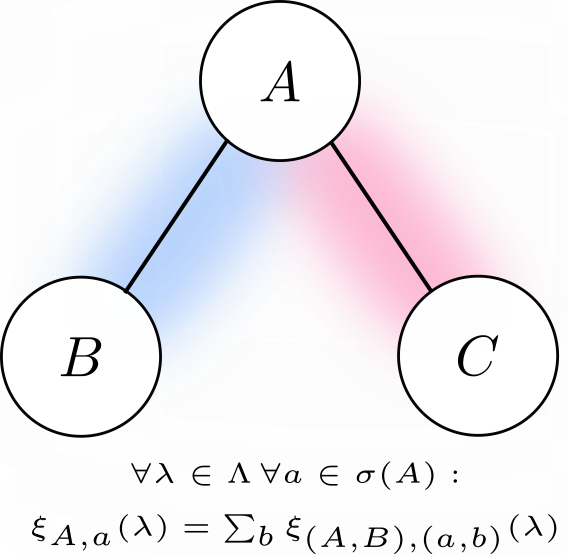
\includegraphics[width=0.4\textwidth]{images/trianglegraph.png}
    \caption{Summary of the notion of KS non-contextuality in terms of Hermitian operators. $A,B$ and $B,C$ are assumed to be commuting operators, whereas $B$ and $C$ do not commute. For every ontic state $\lambda\in\Lambda$, a deterministic non-contextual HVM assigns simultaneous eigenvalues $(a,b)$ to the commuting operators ${A,B}$. Context independence requires that taking the marginal of the joint statistics $\xi_{(A,B),(a,b)}$ must reduce to the single operator assignment $\xi_{A,a}$.}
    \label{fig:trianglegraph}
\end{figure}

An important consequence of Condition 2 in Definition \ref{def:kscontherm} is often coined “functional consistency” \cite{Peres2002}. We will only need and prove the property of “functional consistency” for functional relationships which are polynomial, however it could be extended to smooth functions with a converging (multivariate) Taylor expansion. Note that, strictly speaking, context independence implies Condition 2, as permissible outcomes of joint measurements are by definition simultaneous eigenvalues.

\begin{lemma}[functional consistency]\label{lem:funcconsist}\hfill\break Let $\nu_{\lambda}:\operatorname{Herm}(\mathcal{H})\rightarrow\mathbb{\mathbb{R}}$ be a KS non-contextual value assignment, according to Definition \ref{def:kscontherm}, and let $f:\mathbb{R}^{n}\rightarrow\mathbb{R},\thinspace(x_{1},x_{2},\dots,x_{n})\mapsto f(x_{1},x_{2},\dots,x_{n})$ be a polynomial function in $n$ real variables. Further assume that $f(X_{1},X_{2},\dots,X_{n})=0$ holds as an operator identity among the observables of a pairwise commuting set $\{X_{1},X_{2},\dots,X_{n}\}\subset\operatorname{Herm}(\mathcal{H})$. Here $f(X_{1},X_{2},\dots,X_{n})$ is the operator expression obtained by formally inserting operators $X_{i}$ into the real variables $x_{i}$. Then it must hold that $f(\nu_{\lambda}(X_{1}),\nu_{\lambda}(X_{2}),\dots,\nu_{\lambda}(X_{n}))=0$. 
\end{lemma}

\begin{proof}
By definition, the value assignment $\nu_{\lambda}$ assigns simultaneous eigenvalues to the set of pairwise commuting operators. This means that there exists a joint eigenvector $\mathcal{H}\ni\left|\Psi\right\rangle \neq0$ that corresponds to the eigenvalues assigned by $\nu_{\lambda}$. The operator expression $f(X_{1},X_{2},\dots,X_{n})$ is a sum containing terms of the form $c\prod_{i=1}^{n}X_{i}^{\alpha_{i}}$, with $c\in\mathbb{R}$, $\alpha_{i}\in\mathbb{N}_{0}$. Acting with $f(X_{1},X_{2},\dots,X_{n})$ on the joint eigenvector $\ket{\Psi}$ thus “evaluates” $f$ at $(\nu_{\lambda}(X_{1}),\nu_{\lambda}(X_{2}),\dots,\nu_{\lambda}(X_{n})):$\begin{equation*}
f(X_{1},X_{2},\dots,X_{n})\ket{\Psi} =f(\nu_{\lambda}(X_{1}),\nu_{\lambda}(X_{2}),\dots,\nu_{\lambda}(X_{n}))\ket{\Psi} =0.\end{equation*} This concludes the proof, as $\ket{\Psi}$  is non-zero.
\end{proof}

\begin{corollary}
\label{cor:funcconsist}
Let $X_1$, $X_2$ be arbitrary commuting observables and $\nu_{\lambda}:\operatorname{Herm}(\mathcal{H})\rightarrow\mathbb{R}$ a KS non-contextual value assignment. It holds that:
\begin{enumerate}
\item{$\nu_{\lambda}(X_1+X_2)=\nu_{\lambda}(X_1)+\nu_{\lambda}(X_2)$ \footnote{Compare this to the much stronger assumption made by Neumann in his faulty no-go theorem, namely that this relation must hold for arbitary observables. While this produces a contradiction already in two dimensional Hilbert spaces, the unfounded assumption has been mocked as silly by Mermin \cite{Mermin1993}.}}
\item{$\nu_{\lambda}(X_1X_2)=\nu_{\lambda}(X_1)\,\nu(X_2)$}
\end{enumerate}
\end{corollary}

\begin{proof}\hfill
\begin{enumerate}
\item{Define $X=X_1+X_2$, which commutes with both $X_1$ and $X_2$, and apply Lemma \ref{lem:funcconsist} to the operator identity $X-X_1-X_2=0$.}
\item{$X_1X_2$ is a Hermitian operator that commutes with both $X_1$ and $X_2$. Apply Lemma \ref{lem:funcconsist} to the operator identity $(X_1X_2)-(X_1)(X_2)=0$.}
\end{enumerate}
\end{proof}
Let us now turn to the definition of KS non-contextuality in terms of rays in a projective Hilbert space.

\begin{definition}
\label{def:kscontbasis}
Let $\mathcal{H}$ be the system Hilbert space and represent measurements as in Definition \ref{def:projmntsbasis}. A deterministic HVM is \emph{KS non-contextual} if for all ontic states $\lambda\in\Lambda$ there is a value assignment $\omega_{\lambda}:\mathcal{P}(\mathcal{H})\rightarrow\{0,1\}$ satisfying:
\begin{enumerate}
    \item (context independence)\hfill\break$\forall\ket{\Psi} \in\mathcal{P}(\mathcal{H})$, $\forall$ measurements $\mathcal{M}$ with $\ket{\Psi} \in\mathcal{M}\thinspace:\thinspace \omega_{\lambda}(\ket{\Psi} )=\xi_{\mathcal{M},\ket{\Psi} }(\lambda)$
    \item (exactly one outcome)\hfill\break $\forall$ measurements $\{\ket{\Psi_{i}} \}_{i}\subset\mathcal{P}(\mathcal{H})$ it holds that $\sum_{i}\omega_{\lambda}(\ket{\Psi_{i}})=1$
\end{enumerate}
\end{definition}

The interpretation is as follows: think of a measurement $\{\ket{\Psi_{i}} \}_{i}\subset\mathcal{P}(\mathcal{H})$ as a set of yes/no questions posed to the system. For each outcome $\ket{\Psi_{k}}$, a measurement ``asks” if this is a true property of the system, fixed by its ontic state, and subsequently ``reveals” the answer:

Given the ontic state of the system, a general deterministic HVM simultaneously fixes all possible measurement outcomes via the indicator functions $\xi_{\mathcal{M},k}(\lambda)$. This gives us an assignment similar to that above, with the crucial difference that the value assigned to an outcome $\ket{\Psi_{k}}$  may a priori depend on the measurement (ONB) it is regarded to be part of. This ONB is referred to as the ``measurement context”. For our HVM to be consistent with the interpretation of measurements revealing ``true” properties of the system, an outcome being true or false should not depend on what measurement it is a part of. The assumption of KS non-contextuality imposes that the value assigned to any ray be independent of the measurement context, meaning that a ray appearing in multiple measurements must receive the same valuation by the indicator functions, allowing for a functional dependence on only the ray itself. Lastly, Condition 2 ensures that exactly one measurement outcome corresponds to a true property of the system, which is revealed upon performing the measurement. The key points of Definition \ref{def:kscontbasis} are summarized in Figure \ref{fig:onb}, which depicts two measurement bases, assuming a three dimensional Hilbert space.

\begin{figure}
    \centering
    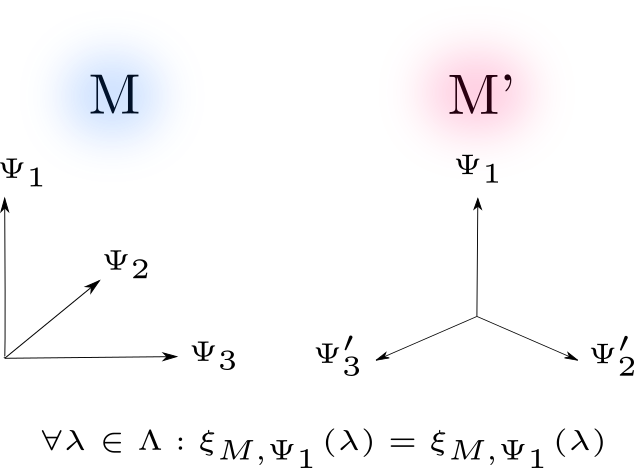
\includegraphics[width=0.5\textwidth]{images/onb.png}
    \caption{Summary of the key points of KS non-contextuality, in terms of vectors in a projective Hilbert space, depicted here to be three-dimensional. The two ONB, $\{\ket{\Psi_1}, \ket{\Psi_2}, \ket{\Psi_3}\}$ and $\{\ket{\Psi_1}, \ket{\Psi_2'}, \ket{\Psi_3'}\}$ are related by a rotation in the plane. As $\ket{\Psi_1}$ appears in both measurements, a non-contextual HVM must assign the same conditional probability of observing the corresponding outcome for every ontic state $\lambda\in\Lambda$.}
    \label{fig:onb}
\end{figure}

As previously stated, both definitions of KS non-contextuality, Definitions \ref{def:kscontherm} and \ref{def:kscontbasis}, are equivalent in the following sense:

\begin{lemma}
\label{lem:equivkscont}
Let $\mathcal{H}$ be a Hilbert space. A non-contextual deterministic value assignment $\hfill\break\omega:\mathcal{P}(\mathcal{H})\rightarrow\{0,1\}$ according to Definition \ref{def:kscontbasis} induces a non-contextual deterministic value assignment $\nu:\operatorname{Herm}(\mathcal{H})\rightarrow\mathbb{\mathbb{R}}$ according to Definition \ref{def:kscontherm}, and vice versa.
\end{lemma}

Lemma \ref{lem:equivkscont} implies that proving the impossibility of a non-contextual deterministic value assignment $\omega:\mathcal{P}(\mathcal{H})\rightarrow\{0,1\}$ for Hilbert spaces of dimension $\geq3$, which we will demonstrate in the next section, entails the impossibility of a non-contextual deterministic HVM according to either definition, as such a HVM would come with a mapping $\nu$ and $\omega$ for every ontic state $\lambda$.

\begin{proof}\emph{(of Lemma \ref{lem:equivkscont})} We prove both implications separately.\begin{itemize}
\item $\nu\Rightarrow\omega$\thinspace: Define $\omega(\left|\Psi\right\rangle )\coloneqq\nu(\left|\Psi\right\rangle \left\langle \Psi\right|)$. Projectors $\left|\Psi\right\rangle \left\langle \Psi\right|$ have eigenvalues {0,1}, therefore $\omega$ maps to $\{0,1\}$. Since orthogonal projectors commute, by the property of ``functional consistency", in particular Corollary \ref{cor:funcconsist}, we get:
\begin{equation*}
    \{\left|\Psi_{i}\right\rangle \}_{i}\subset\mathcal{H} \text{ an ONB } \Rightarrow\sum_{i}\omega(\left|\Psi_{i}\right\rangle )=\sum_{i}\nu(\left|\Psi_{i}\right\rangle \left\langle \Psi_{i}\right|)=\nu(\sum_{i}\left|\Psi_{i}\right\rangle \left\langle \Psi_{i}\right|)=\nu(\mathbb{1}_{\mathcal{H}})=1.\end{equation*}

\item $\omega\Rightarrow\nu$: (Adapted from \cite{Pusey2019}) Define $\nu(A=\sum_{i,j}a_{i}|\Psi_{j}^{(i)}\rangle\langle\Psi_{j}^{(i)}|)\coloneqq\sum_{i,j}a_{i}\thinspace\omega(|\Psi_{j}^{(i)}\rangle)$, where we have used that every Hermitian operator can be spectrally decomposed. We take the eigenvalues $a_{i}$ to be distinct, $\{|\Psi_{j}^{(i)}\rangle\}_{j}$ being an ONB of the eigenspace corresponding to the eigenvalue $a_{i}$. The spectral decomposition of a Hermitian operator is not unique, as we may choose different ONB of the eigenspaces, in case of degeneracies. Nonetheless the above assignment is well-defined: Take
\begin{equation*}
    A=\sum_{i,j}a_{i}|\Psi_{j}^{(i)}\rangle\langle\Psi_{j}^{(i)}|=\sum_{i,j}a_{i}|\Phi_{j}^{(i)}\rangle\langle\Phi_{j}^{(i)}|
\end{equation*}
to be two spectral decompositions of $A$. Both $\{|\Psi_{j}^{(i)}\rangle\}_{j}$ and $\{|\Phi_{j}^{(i)}\rangle\}_{j}$ span the eigenspace corresponding to the eigenvalue $a_{i}$. We can extend both subsets to ONB of $\mathcal{H}$ by adding an orthonormal set $\{|\Theta_{k}\rangle\}_{k}$ to each. By the defining property of $\omega$ we get
\begin{equation*}
    \sum_{j}\omega(|\Psi_{j}^{(i)}\rangle)=\sum_{j}\omega(|\Phi_{j}^{(i)}\rangle)
\end{equation*} 
for all i, which means that $\nu$ is well-defined. Suppose $\{A,B,...\}\subset\operatorname{Herm}(\mathcal{H})$ is a set of mutually commuting Hermitian operators. There exists a shared ONB of eigenvectors $\{\left|\Psi_{i}\right\rangle \}_{i}$. Let 
\begin{align*}
    A & =\sum_{i}a_{i}\left|\Psi_{i}\right\rangle \left\langle \Psi_{i}\right| \text{ and } B =\sum_{i}b_{i}\left|\Psi_{i}\right\rangle \left\langle \Psi_{i}\right|
\end{align*}
be spectral decompositions of $A$ and $B$, where the eigenvalues $a_{i}$, $b_{i}$ can now be repeating. The assignment $\nu$ maps $A$ and $B$ to
\begin{align*}
    \nu(A) =\sum_{i}a_{i}\,\omega(\left|\Psi_{i}\right\rangle ) \text{ and } \nu(B)  =\sum_{i}b_{i}\,\omega(\left|\Psi_{i}\right\rangle ).
\end{align*}
Thus, commuting operators are mapped to simultaneous eigenvalues, and $\nu$ is a KS non-contextual value assignment like in Definition \ref{def:kscontherm}.
\end{itemize}
\end{proof}

\section{Formal statement and proof of the KS Theorem}
\label{sec:formalproof}

The KS Theorem was first proved by Kochen and Specker in 1968 \cite{Kochen1968}. Previously, Bell independently proved that a deterministic HVM of QM that induces a non-contextual value assignment like in Definition \ref{def:kscontbasis}, must be contextual \cite{Bell1966}. However his proof was deemed less convincing, as it used a continuum of vector directions, as opposed to an explicit finite set \cite{Mermin1993}.

We are now ready to reformulate the KS Theorem in precise mathematical terms (adapted from \cite{Pusey2019}):

\begin{theorem}[Kochen-Specker \cite{Kochen1968}]\hfill\break
\label{thm:ksthm}
For all projective Hilbert spaces $\mathcal{P}(\mathcal{H})$ of dimension $\geq3$, there exists a finite set $S\subset\mathcal{P}(\mathcal{H})$ of rays for which no valid value assignment $\omega:S\rightarrow\{0,1\}$ exists, satisfying the conditions for a KS non-contextual model, according to Definition \ref{def:kscontbasis}.
\end{theorem}

The existence of such a set $\mathcal{S}$ is in contradiction with any attempt of a KS non-contextual deterministic HVM of QM, as KS non-contextuality implies a valid value assignment for every possible ontic state of the system. Thus the KS Theorem effectively states the impossibility of a non-contextual deterministic HVM. 

As Pusey notes \cite{Pusey2019}, all assumptions (outcome determinism, context independence and Hilbert spaces of dimension $\ge3$) of the KS Theorem are necessary for the proof of impossibility. If we allow for context dependence, such a value assignment can be given for all sets $\mathcal{S}$, as we can assign appropriate values for each measurement contained in $\mathcal{S}$. Furthermore, relaxing the assumption of outcome determinism to an assignment of probabilities $\tilde{\omega}:\mathcal{S}\rightarrow\left[0,1\right]$ spoils the proof of impossibility, as a valid value assignment $\tilde{\omega}$ is given for instance by the Born rule: $\tilde{\omega}(\ket{\Psi_{i}} )\coloneqq\operatorname{tr}(\rho\ket{\Psi_{i}} \bra{\Psi_{i}})$ for some non-negative (Hermitian) operator $\rho$ with $\operatorname{tr}(\rho)=1$. Lastly, for Hilbert spaces of dimension 2, it is possible to give an explicit form of a non-contextual deterministic HVM \cite{Mermin1993}. The deeper reason for why our proof does not extend to the two-dimensional case is that it makes heavy use of overlapping ONB (measurement contexts) in the construction of $\mathcal{S}$, meaning different measurements that share at least one ray. These will be key in establishing a contradiction for dimensions $\geq3$. However, for two-dimensional Hilbert spaces, it is impossible to construct overlapping and distinct ONB, as a single ray fixes the ONB.

The proof of the KS Theorem is by induction with respect to to the dimension. The following Lemma (induction step), once proven, reduces the proof of the KS Theorem to the three-dimensional base case. We will prove the three-dimensional base case by giving an explicit set of directions belonging to overlapping orthogonal triads, for which a KS non-contextual value assignment can be shown to be impossible. This will be demonstrated by a chain of geometric arguments.

\begin{lemma}[\cite{Pusey2019}]\hfill\break
Assume that all projective Hilbert spaces of dimension d have a finite subset like in the KS Theorem. Let $\mathcal{P}(\mathcal{H})$ be a projective Hilbert space of dimension d+1. Then $\exists\thinspace\mathbb{\mathcal{S}\in\mathcal{P}}(\mathcal{H})$ with the same properties. 
\end{lemma}

\begin{proof}
We follow \cite{Pusey2019}. Let $\{\ket{0},\dots,\ket{d} \}$ be an ONB of $\mathcal{H}$ and let $\mathcal{H}_{0}$, $\mathcal{H}_{1}\subset\mathcal{H}$ be the d-dimensional subspaces orthogonal to $\ket{0}$, $\ket{1}$, respectively. There exist subets $\mathcal{S}_{0}$, $\mathcal{S}_{1}$ of $\mathcal{P}(\mathcal{H}_{0})$, $\mathcal{P}(\mathcal{H}_{1})$, for which there are no valid value assignments within the respective projective Hilbert space. Let $\mathcal{S}_{0}'$, $\mathcal{S}_{1}'$ denote the embeddings of $\mathcal{S}_{0}$, $\mathcal{S}_{1}$ into $\mathcal{H}$. We will show that $\mathcal{S}'\coloneqq\mathcal{S}_{0}'\cup\mathcal{S}_{1}'\cup\{\ket{0},\dots, \ket{d}\}$ then defines a subset of $\mathcal{P}(\mathcal{H})$ for which there is no valid non-contextual value assignment. As $\{\ket{0},\dots,\ket{d} \}$ constitutes an ONB, a valid value assignment $\omega'$ has to map $\ket{0}$ or $\ket{1}$  (or both) to 0. Both $\omega'(\ket{0})=0$ and $\omega'(\ket{1})=0$ lead to a contradiction: For instance, say $\omega'(\ket{0})=0$. For any ONB $\mathcal{M}\subset\mathcal{H}_{0}$ and its embedding $\mathcal{M'}\subset\mathcal{H}$ we have
\begin{equation*}
\sum\limits _{\ket{\Psi_{i}}\in M'}\omega'(\left|\Psi_{i}\right\rangle )+\omega'(\ket{0} )=\sum\limits _{\ket{\Psi_{i}}\in M'}\omega'(\ket{\Psi_{i}})=1.     
\end{equation*}
Hence, $\omega:\mathcal{S}_{0}\mapsto\{0,1\}$, $\omega(\ket{\Psi} )\coloneqq\omega'(\ket{\Psi'})$ satisfies Condition 2 of \ref{def:kscontbasis}, where $\ket{\Psi'} \in\mathcal{S}_{0}'$ is the embedding of $\ket{\Psi} \in\mathcal{S}_{0}$ into $\mathcal{H}$. As per assumption, $w$ cannot be context independent. Therefore, by extension, $w'$ must also be context dependent.
\end{proof}
What remains is a proof for the existence of a finite subset $\mathcal{S}$ that does not permit a valid KS non-contextual value assignment for the case of three dimensions. The following lemma allows us to consider only the three-dimensional complex projective space $\mathcal{P}(\mathbb{C}^{3})$ w.l.o.g.:

\begin{lemma}
Let $\mathcal{H}_{n}$ be a n-dimensional dimensional complex Hilbert space. A valid KS non-contextual value assignment $\omega:\mathcal{P}(\mathcal{H}_{n})\rightarrow\{0,1\}$ according to Definition \ref{def:kscontbasis} induces a valid value assignment $\tilde{\omega}:\mathcal{P}(\mathbb{C}^{n})\rightarrow\{0,1\}$.
\end{lemma}

\begin{proof}
Let $\{\left|\Psi_{i}\right\rangle \}_{i\in\{1,\dots,n\}}$ be an ONB of $\mathcal{H}_{n}$. We can construct the isomorphism $\mathcal{J}:\mathcal{\mathcal{H}}_{n}\rightarrow\mathbb{C}^{n}$, $\ket{\Psi_{k}} \mapsto e_{k}$ , where $\{e_{i}\}_{i\in\{1,\dots,n\}}$ is the standard basis of $\mathbb{C}^{n}$. This isomorphism preserves the inner product structure, as it maps an ONB of $\mathcal{H}_{n}$ to an ONB of $\mathbb{C}^{n}$. Thus, $\mathcal{J}$ preserves all orthogonality relations. A valid non-contextual value assignment according to Definition \ref{def:kscontbasis} then induces a valid non-contextual value assignment $\tilde{\omega}:\mathcal{P}(\mathbb{C}^{n})\rightarrow\{0,1\}$ via $\tilde{\omega}\coloneqq\omega\circ\mathcal{J}^{-1}$.
\end{proof}

Having reduced the proof of the three-dimensional base case to proving the impossibility of a valid non-contextual value assignment $\tilde{\omega}:\mathcal{P}(\mathbb{C}^{3})\rightarrow\{0,1\}$, we will now turn our attention to this task. Lemma \ref{lem:3dbasecase} sticks to Peres' notation \cite{Peres1991} for saving space:

\begin{lemma}
\label{lem:3dbasecase}
Let $\bar{1}$ denote -1 and 2 denote $\sqrt{2}$. For the following set of 33 vectors $\mathcal{S}\subset\mathbb{R}^{3}\subset\mathbb{C}^{3}$ (“Peres configuration” \footnote{For a nice visualization of the “Peres configuration”, see Conway and Kochen's paper “The Strong Free Will Theorem”, which also makes use of it \cite{Conway2011}.} \cite{Peres1991}) it is impossible to assign values $\{0,1\}$ to each vector such that for all orthogonal triads contained in $\mathcal{S}$ exactly one member receives the valuation 1:
\begin{equation*}
\begin{split}
\mathcal{S}= \{ & 100,010,001,110,101,011,1\bar{1}0,\bar{1}01,0\bar{1}1,1\bar{1}2,\bar{1}12, \\
& \bar{2}01,021,102,\bar{2}11,211,\bar{1}02,201,\bar{1}\bar{1}2,112,0\bar{2}1,012, \\
& 1\bar{2}1,121,0\bar{1}2,12\bar{1},\bar{1}21,21\bar{1},2\bar{1}1,\bar{2}10,1\bar{2}0,120,210\} 
\end{split}
\end{equation*}
Here, the tuple $\bar{2}01$ for instance corresponds to the vector 
$\begin{pmatrix}
\text{-}\sqrt{2}\\
0\\
1
\end{pmatrix}\in\mathbb{R}^{3}.$
\end{lemma}

We consider unnormalized vectors only for convenience as this does not affect orthogonality relations. 

The cubic symmetry of the set $\mathcal{S}$ greatly simplifies the proof. More precisely, the set $\mathcal{S}$ is invariant under interchange of the $x,y,z$ axes and under a reversal of the direction of each axis $x\mapsto\bar{x}$. It is the case that \begin{equation*}
\omega:\mathbb{\mathcal{S}\rightarrow}\{0,1\}\text{ is a valid value assignment}\iff\omega\circ T\text{ is a valid value assignment,}\end{equation*}
$T$ being one of the aforementioned symmetry transformations. This is straightforward to see, as the symmetry transformations of $\mathcal{S}$ are orthogonal transformations that leave orthogonality relations unchanged. The following concrete example shows how we can exploit the symmetry of $\mathcal{S}$ to make arbitrary assignments w.l.o.g.: Consider the orthogonal triad $\{001,100,010\}$. Assuming there exists a valid value assignment $\omega:\mathbb{\mathcal{S}\rightarrow}\{0,1\}$, then exactly one of the three vectors in the triad is assigned a 1. Due to the symmetry of the set $\mathcal{
S}$, there must be a valid value assignment $\omega'$ that assigns 001 the value 1. Analogous considerations apply to symmetry transformations $x\mapsto\bar{x}$. 

On a historical note, the original KS paper \cite{Kochen1968} gives an explicit set of 117 directions in $\mathbb{R}^{3}$ that lead to a contradiction. The current record holders are Kochen and Conway, with a set of 31 directions, however their set is not as highly symmetric as the Peres configuration, which complicates the proof \cite{Peres2002}.

\begin{proof} \emph{(of Lemma \ref{lem:3dbasecase})}\hfil\break
The proof of Lemma \ref{lem:3dbasecase} is given by the table in Figure \ref{fig:ksproof} and shows that any attempt to construct a valid KS non-contextual value assignment $\omega:\mathbb{\mathcal{S}\rightarrow}\{0,1\}$ inevitably leads to a contradiction. Finding such an assignment is equivalent to a colouring problem. Identifying 1 $\equiv$ ``green'', 0 $\equiv$ ``red'', a valid value assignment corresponds to a colouring of the rays in $\mathcal{S}$, in accordance with with the rule that each orthogonal triad in $\mathcal{S}$ must have exactly one element coloured green and two elements coloured red. Such a colouring of rays is shown to be impossible, making use of the fact that $\mathcal{S}$ contains rays that are part of multiple distinct orthogonal triads. Each line of the table introduces a new orthogonal triad that is coloured, either w.l.o.g.\ , making use of the symmetry of $\mathcal{S}$, or according to the values of previous triads. In each line, only the first ray of the triad is coloured green. The “Other rays” in each line are orthogonal to the single green ray in that line and are consequently coloured red. The stepwise colouring of rays leaves the set $\{100,021,0\text{\ensuremath{\bar{1}}2}\}$ coloured red. As these rays form an orthogonal triad, this proves that a valid colouring and thus a valid value assignment are impossible.
\end{proof}

\begin{figure}
\centering
\begin{subfigure}{\textwidth}
\centering
 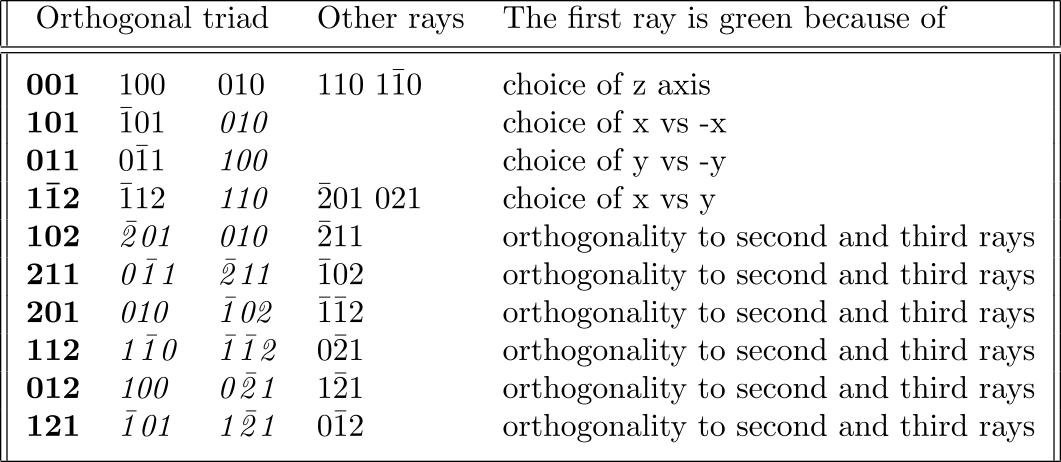
\includegraphics[width=\textwidth]{images/perestable.png}
 \caption{Table containing the proof of the three-dimensional base case of the KS Theorem, in terms of a colouring problem where each orthogonal triad must contain exactly one green and two red rays. Each line of the table introduces a new orthogonal triad that is coloured, either w.l.o.g.\ or according to the values of previous triads. In each line, only the first ray of the triad is coloured green. The ``Other rays'' in each line are orthogonal to the single green ray in that line and are consequently coloured red. The stepwise colouring of rays leaves the orthogonal triad \{100,021,0\text{$\bar{1}$2}\} coloured red, proving the impossiblity of a valid colouring. Table copied from \cite{Peres1991}.}
 \label{fig:table}
\end{subfigure}
\hfill\break
\begin{subfigure}{\textwidth}
\centering
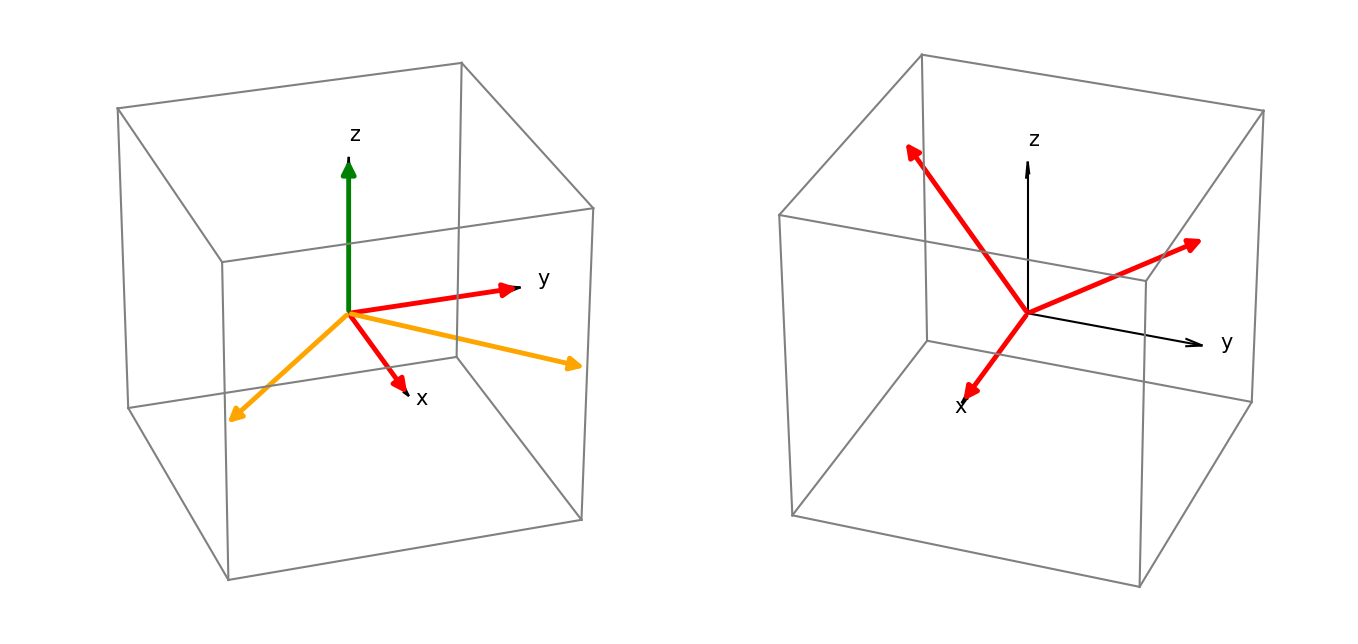
\includegraphics[width=\textwidth]{images/triads.png}
\caption{The left plot visualizes the first line of the proof-containing table, ``Other rays'' being coloured orange. The right plot visualizes the resulting contradiction, refer to the text.}
\label{fig:triads}
\end{subfigure}
\caption{Proof of the KS Theorem}
\label{fig:ksproof}
\end{figure}

\section{Algebraic proof in four dimensions}
\label{sec:4dim}
We now reap the fruits of our previous efforts that proved the equivalence of KS non-contextual value assignments to rays and such assignments to Hermitian operators. This allows us to give a far simpler and purely algebraic proof of the KS Theorem in four dimensions, which uses KS non-contextuality in terms of Hermitian operators. For the same reasons as in three dimensions, we can w.l.o.g.\ assume $\mathcal{H=\mathbb{C}}^{4}\cong\mathbb{C}^{2}\otimes\mathbb{C}^{2}$ \footnote{This is not to say that we are now considering two remote systems, but only provides a convenient way to define the set of operators used in the proof.}. Consider the set of operators depicted in Figure \ref{fig:4dim}. They form the so-called “Mermin Square” \cite{Mermin1993} and can be written in terms of Pauli operators. The operators are arranged such that the operators in each of the three rows, columns are mutually commuting. Additionally, the product of the three observables in the rightmost column is $-\mathbb{1}_{\mathbb{C}^{2}\otimes\mathbb{C}^{2}}$. The product of the three observables in all other columns and all rows is $+\mathbb{1}_{\mathbb{C}^{2}\otimes\mathbb{C}^{2}}$. By Corollary \ref{cor:funcconsist}, a KS non-contextual value assignment assigns values to the operators such that the product of values within one row, column is $\pm1$, in accordance with the corresponding operator identities. It follows that, by the row identities, the product of all nine values is $+1$, whereas the column identities result in a value of $-1$, a contradiction.

\begin{figure}
    \centering
    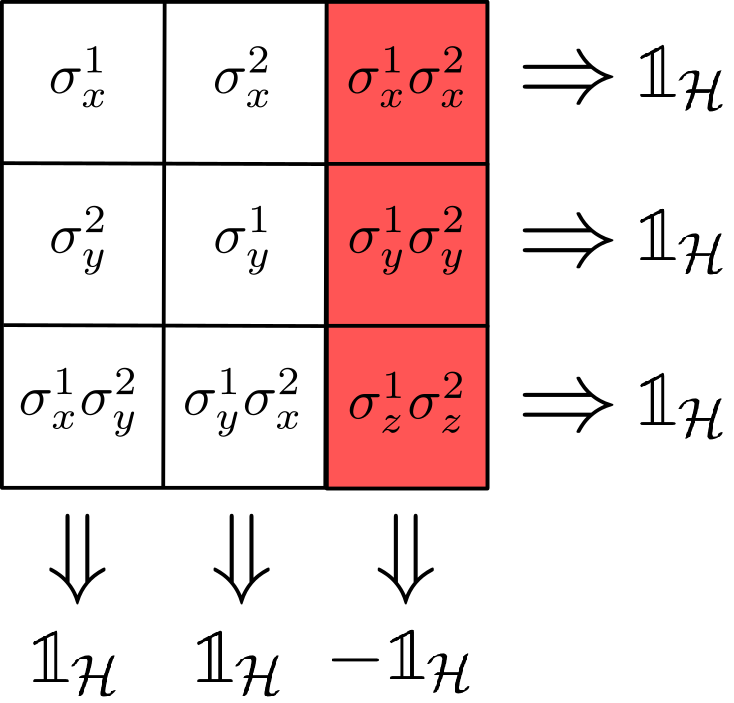
\includegraphics[width=0.5\textwidth]{images/4dim.png}
    \caption{``Mermin Square'': Operators on $\mathbb{C}^{2}\otimes\mathbb{C}^{2}$ that allow for a proof of the KS Theorem in four dimensions. Tensor products between Pauli operators are omitted for readability. Within each row and each column, the operators commute. A non-contextual value assignment to these operators is contradictory, in the sense that the product of all nine values assigned to the operators would not be well-defined. For each row, the product of the three operators in that row is $\mathbb{1}_\mathcal{H}$. The same holds for the columns, with the notable exception that the product of the three operators in the rightmost column is $-\mathbb{1}_\mathcal{H}$. These identities on an operator level are key in establishing a contradiction. Figure adapted from \cite{Mermin1993}.}
    \label{fig:4dim}
\end{figure}

\section[Local causality and Bell's Theorem\\ Locality as an instance of KS]{Local causality and Bell's Theorem\\ \large{Locality as an instance of contextuality}}

\label{sec:bell}
The following is meant to discuss the relationship between the KS Theorem and Bell's Theorem, in particular the connection between KS non-contextuality and Bell's notion of local causality. 

Consider the well-known CHSH (thought-)experiment \cite{Clauser1969,Colbeck2019,Spekkens2012} that proves QM to be incompatible with a local HVM description. In particular, quantum theory predicts violations of the CHSH Bell inequality, which must be satisfied for all local HVM.

A source S emits pairs of entangled particles in the state $\left|\Psi\right\rangle =\frac{1}{\sqrt{2}}(\ket{\uparrow\uparrow} +\ket{\downarrow\downarrow})$ (EPR pairs) that split up and travel to two remote labs. In each of the labs, an experimenter can choose between two incompatible two-outcome measurements $A_{1}$, $A_{2}$ and $B_{1}$, $B_{2}$, respectively. One can for instance think of these as measuring different spin components of the particle. We will label the outcomes with $\pm1$. The setting of the CHSH experiment is shown in Figure \ref{fig:bell}. Let $X$, $Y$ be random variables that describe the measurement outcomes of $A_i$, $B_i$, respectively. For uniformly chosen detector settings, we wish to measure the probability
\begin{equation*}
\begin{split}
p(\text{{success}}) =\thinspace & p(X=Y,A_1,B_1)+p(X=Y,A_2,B_1) \\
& p(X=Y,A_2,B_2)+p(X\neq Y,A_1,B_2),
\end{split}
\end{equation*}
as is illustrated in Figure \ref{fig:chsh}.
All correlations compatible with a general HVM description must be of the form
\begin{equation*}
p(X=x,Y=y,A_i,B_j)=\int_{\Lambda}d\lambda\thinspace\mu(\lambda)\,p(X=x,Y=y\vert A_i,B_j,\lambda)\,p(A_i,B_j\vert \lambda),
\end{equation*}
where $\mu$ is some probability density function on the ontic state space $\lambda$.
Driven by special relativity, we further assume local causality to be a property of all valid classical descriptions: Rewriting $p(X=x,Y=y \vert A_i,B_j,\lambda)$ as $p(X=x\vert A_i, B_j, Y=y, \lambda)p(Y=y\vert A_i,B_j,\lambda)$, local causality is the assumption that, given a complete specification of the ontic state $\lambda$, the outcome of a measurement is independent of what other measurements are performed in a space-like separated region of space-time, as well as their outcomes:
\begin{align*}
    p(X=x\vert A_i,B_j,Y,\lambda) & =p(X=x\vert A_i,\lambda) \\
    p(Y=y\vert A_i,B_j,\lambda) & =p(Y=y\vert B_j,\lambda)
\end{align*}
For any ontological model of reality, local causality provides the best and most natural explanation for the fact that such superluminal influences have never been observed in experiments. Analogously, KS non-contextuality provides the most natural explanation for why, within the framework of QM, compatible observables do not disturb each other's outcome statistics. We will revisit this point in Section \ref{sec:spekkcont}, where we introduce a revised notion of contextuality due to Spekkens.
All correlations compatible with a local HVM description, i.e.\ an ontological model obeying local causality, must be of the form
\begin{equation*}
p(X=x,Y=y\vert A_i,B_j)=\int_{\Lambda}d\lambda\thinspace\mu(\lambda)p_{A}(X=x\vert A_i, \lambda)p_{B}(Y=y\vert B_j, \lambda).
\end{equation*}
The assumption of local causality for the space-like separated regions A and B manifests itself in the local response functions $p_A$ and $p_B$. W.l.o.g.\ , we can assume $p_A$ and $p_B$ to be deterministic response functions, as we may shift all classical randomness into the ontic states and the distribution $\mu$ over these. This is sometimes referred to as Fine's Theorem \cite{Fine1982}. Importantly, Fine's Theorem does not hold for general contextuality scenarios without space-like separated subsystems, as for two compatible local operators $A$, $A'$, the set of simultaneous eigenvalues is in general not given by the Cartesian product $\sigma(A)\times\sigma(A')$. We will discuss complications that arise without space-like separated subsystems in Section \ref{sec:complicationscont}.

Assuming that the experimenters can choose the detector settings freely (no super-determinism), the choice of measurement should not be correlated with the ontic state $\lambda$ emitted by the source. Therefore, $p(A_i,B_j\vert \lambda)=p(A_i,B_j)$. All in all, for the CHSH experiment\footnote{This can of course be extended to more general correlation experiments in a Bell-like setting.} to have a valid classical \textbf{HVM description} obeying \textbf{local causality} and the assumption of \textbf{freely random detector settings}, chosen according to a \textbf{uniform distribution}, all correlations must be of the form:
\begin{equation}
\label{eqn:lhvm}
p(X=x,Y=y,A_i,B_j)=\frac{1}{4}\int_{\Lambda}d\lambda\thinspace\mu(\lambda)p_{A}(X=x\vert A_i, \lambda)p_{B}(Y=y\vert B_j, \lambda),
\end{equation}
where $p_A$ and $p_B$ are deterministic probability assignments.

Given the general expression for correlations, as prescribed by a local HVM description \ref{eqn:lhvm}, it immediately follows that $p(\text{{success}})$ is upper-bounded by $\frac{3}{4}$ for any such HVM description. This can be verified in the same manner as in Section \ref{sec:threeboxes}, where we showed deterministic and non-contextual HVM descriptions to be incompatible with Specker's three boxes: Examining Figure \ref{fig:chsh}, we realize that there is no deterministic assignment of measurement outcomes $\pm 1$ to the four measurement operators, such that all ``winning" correlations are satisfied. In fact, for any such assignment, at most three of the four ``winning" correlations are satisfied. The local response functions in Equation \ref{eqn:lhvm} induce such a deterministic assignment. Therefore, for every ontic state $\lambda$, $p(\text{success})$ is upper-bounded by $\frac{3}{4}$. The ensemble average over all ontic states $\lambda\in\Lambda$ is thus upper-bounded by the same quantity.
Consequently, $p(\text{{success}})\leq\frac{3}{4}$ is a Bell inequality: the so-called \textbf{CHSH Bell-inequality} \cite{Clauser1969,Colbeck2019,Spekkens2012}:
\begin{equation}
    \label{eqn:chshineq}
    p(\text{success}) = p(X=Y,A_1,B_1)+p(X=Y,A_2,B_1)+p(X=Y,A_2,B_2)+p(X\neq Y,A_1,B_2)\leq \frac{3}{4}
\end{equation}

In QM, outcome probabilities are computed according to the Born rule. Assuming projective measurements on a pure quantum state, permissible quantum correlations for Bell-type experiments are of the form
\begin{equation*}
p(X=x,Y=y\vert A_i, B_j)=\expval{\Pi_{A_i}^x\otimes\Pi_{B_j}^y}{\Psi},
\end{equation*}
where $\ket{\Psi}\in\mathcal{H}$ is a normalized, bipartite Hilbert state vector and $\Pi_{A_i}^x$ is the projection operator corresponding to the outcome $x$ of the measurement $A_i$ on the subsystem A.

What is remarkable about the CHSH scenario is the fact that one can give explicit projective measurements $A_{1}$, $A_{2}$, $B_{1}$, $B_{2}$, as well as the maximally entangled pure state $\ket{\Psi} =\frac{1}{\sqrt{2}}(\ket{\uparrow\uparrow} +\ket{\downarrow\downarrow})$, for which quantum theory predicts $p(\text{{success}})=\cos^{2}(\frac{\pi}{8})>\frac{3}{4}$: a violation of the CHSH Bell inequality. A set of Hermitian operators with this property is 
\begin{equation}
\label{eqn:chshmnts}
\begin{split}
A_{1} & =\ket{0}\bra{0}-\ket{\pi}\bra{\pi},\\
A_{2} & =|\frac{\pi}{2}\rangle\langle\frac{\pi}{2}|-|\frac{3\pi}{2}\rangle\langle\frac{3\pi}{2}|,\\
B_{1} & =|\frac{\pi}{4}\rangle\langle\frac{\pi}{4}|-|\frac{5\pi}{4}\rangle\langle\frac{5\pi}{4}|,\\
B_{2} & =|\frac{3\pi}{4}\rangle\langle\frac{3\pi}{4}|-|\frac{7\pi}{4}\rangle\langle\frac{7\pi}{4}|,
\end{split}
\end{equation}
with $\ket{\theta} \coloneqq\cos(\frac{\theta}{2})\ket{\uparrow} +\sin(\frac{\theta}{2})\ket{\downarrow}$ \cite{Colbeck2019}. Recall that we label the two distinct measurement outcomes with the eigenvalues $\pm 1$. Each local measurement projects the state of the particle on which it acts onto one of two antipodal surface points in the xz-plane of the single qubit Bloch sphere. As the two particles are entangled, in particular maximally correlated, measuring one particle will ``steer" the state of the other particle\footnote{This does not violate the no-signalling principle, as can be seen by computing the reduced density operator of system B: it describes a maximally mixed state.}. Thus, the probability of the measurements $(A_1,B_2)$ yielding anti-correlated outcomes is given by $\frac{1}{2}\abs{\bra{0}\ket{\frac{7\pi}{4}}}^2+\frac{1}{2}\abs{\bra{\pi}\ket{\frac{3\pi}{4}}}^2=\cos^2(\frac{\pi}{8})$. In fact, for each of the four possible measurement settings, the probability of the measurement outcomes being related as in Figure \ref{fig:chsh} is $\cos^2(\frac{\pi}{8})$. To see this, recall that we may associate with each local measurement outcome a point on the Bloch sphere, and by extension with every local measurement operator an axis connecting two antipodal points on the Bloch sphere, as shown in Figure \ref{fig:chshmnts}. These axes are rotated by an angle of $\frac{\pi}{4}$ (in real space) relative to one another and lie within the xz-plane. For all $A_i$ and $B_j$, the measurement operators are chosen in such a way that the overlap of the Bloch states corresponding to measurement outcomes that obey the correlations in Figure \ref{fig:chsh} is $\cos(\frac{\pi}{8})$.

\begin{figure}
\centering
\begin{subfigure}{\textwidth}
\centering
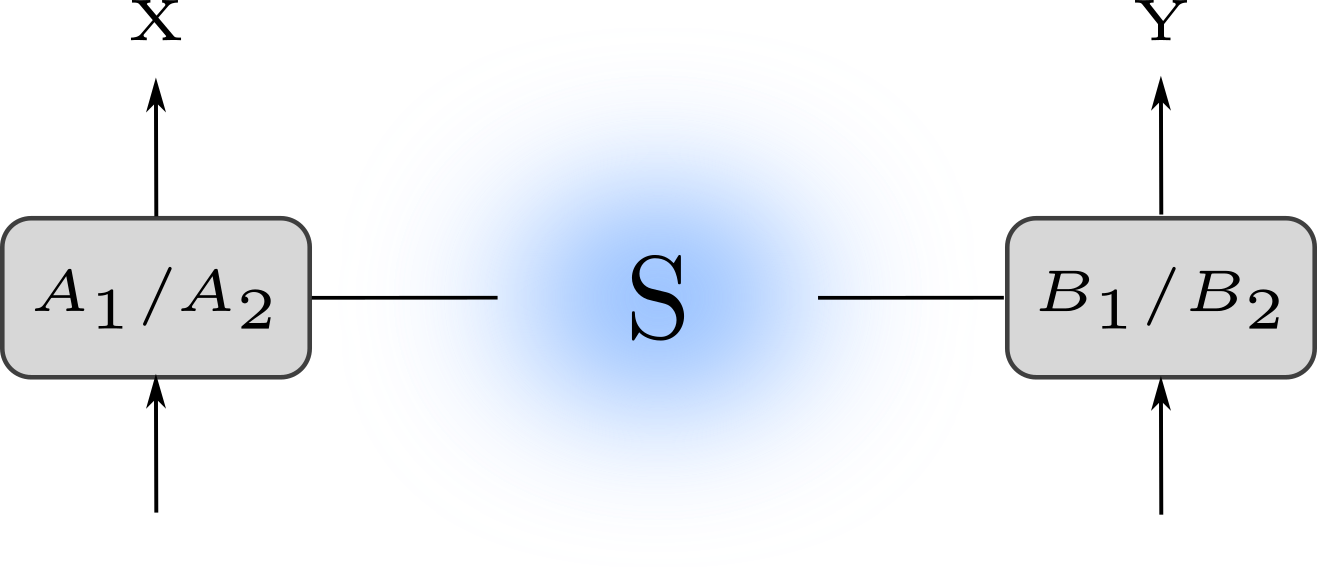
\includegraphics[width=0.7\textwidth]{images/bell.png}
\caption{CHSH setup leading to violations of the CHSH inequality. A source $S$ emits entangled EPR pairs. Constituent particles are measured in space-like separated regions, with experimenters being able to choose between two incompatible measurements $A_1$, $A_2$ or $B_1$, $B_2$. The random variables X, Y hold the measurement outcome for operators $A_1, A_2$ or $B_1, B_2$, respectively.\\[1em]}
\label{fig:bell}
\end{subfigure}
\begin{subfigure}{\textwidth}
\centering
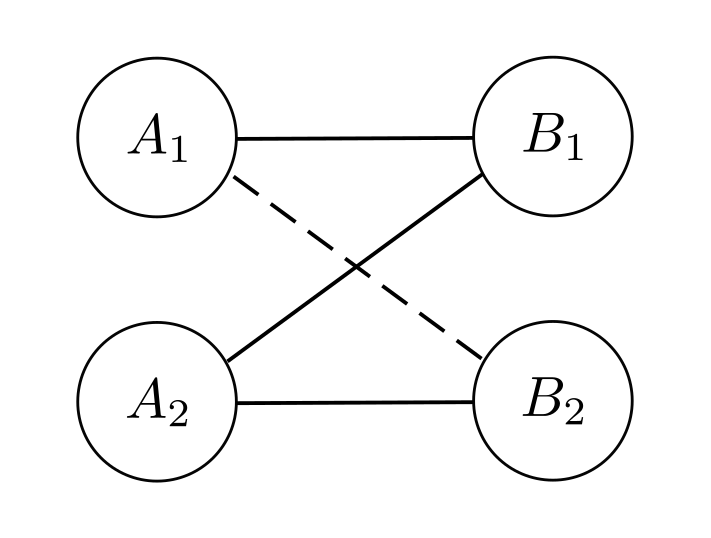
\includegraphics[width=0.4\textwidth]{images/chsh.png}
\caption{CHSH correlations for space-like separated operators $A_1$, $A_2$ and $B_1$, $B_2$. Lines indicate joint measurability. A solid line further indicates correlated outcomes, whereas a dashed line indicates anti-correlated outcomes. Let $X$, $Y$ be random variables that describe the measurement outcomes of $A_i$, $B_i$, respectively. We are interested in the probability that $X=Y$ for all choices of measurements but $(A_1,B_2)$ and $X\neq Y$ for the measurements $(A_1,B_2)$. Adapted from \cite{Spekkens2012}.\\[1em]}
\label{fig:chsh}
\end{subfigure}
\caption{CHSH Bell test}
\label{fig:chshbelltest}
\end{figure}

\begin{figure}
    \centering
    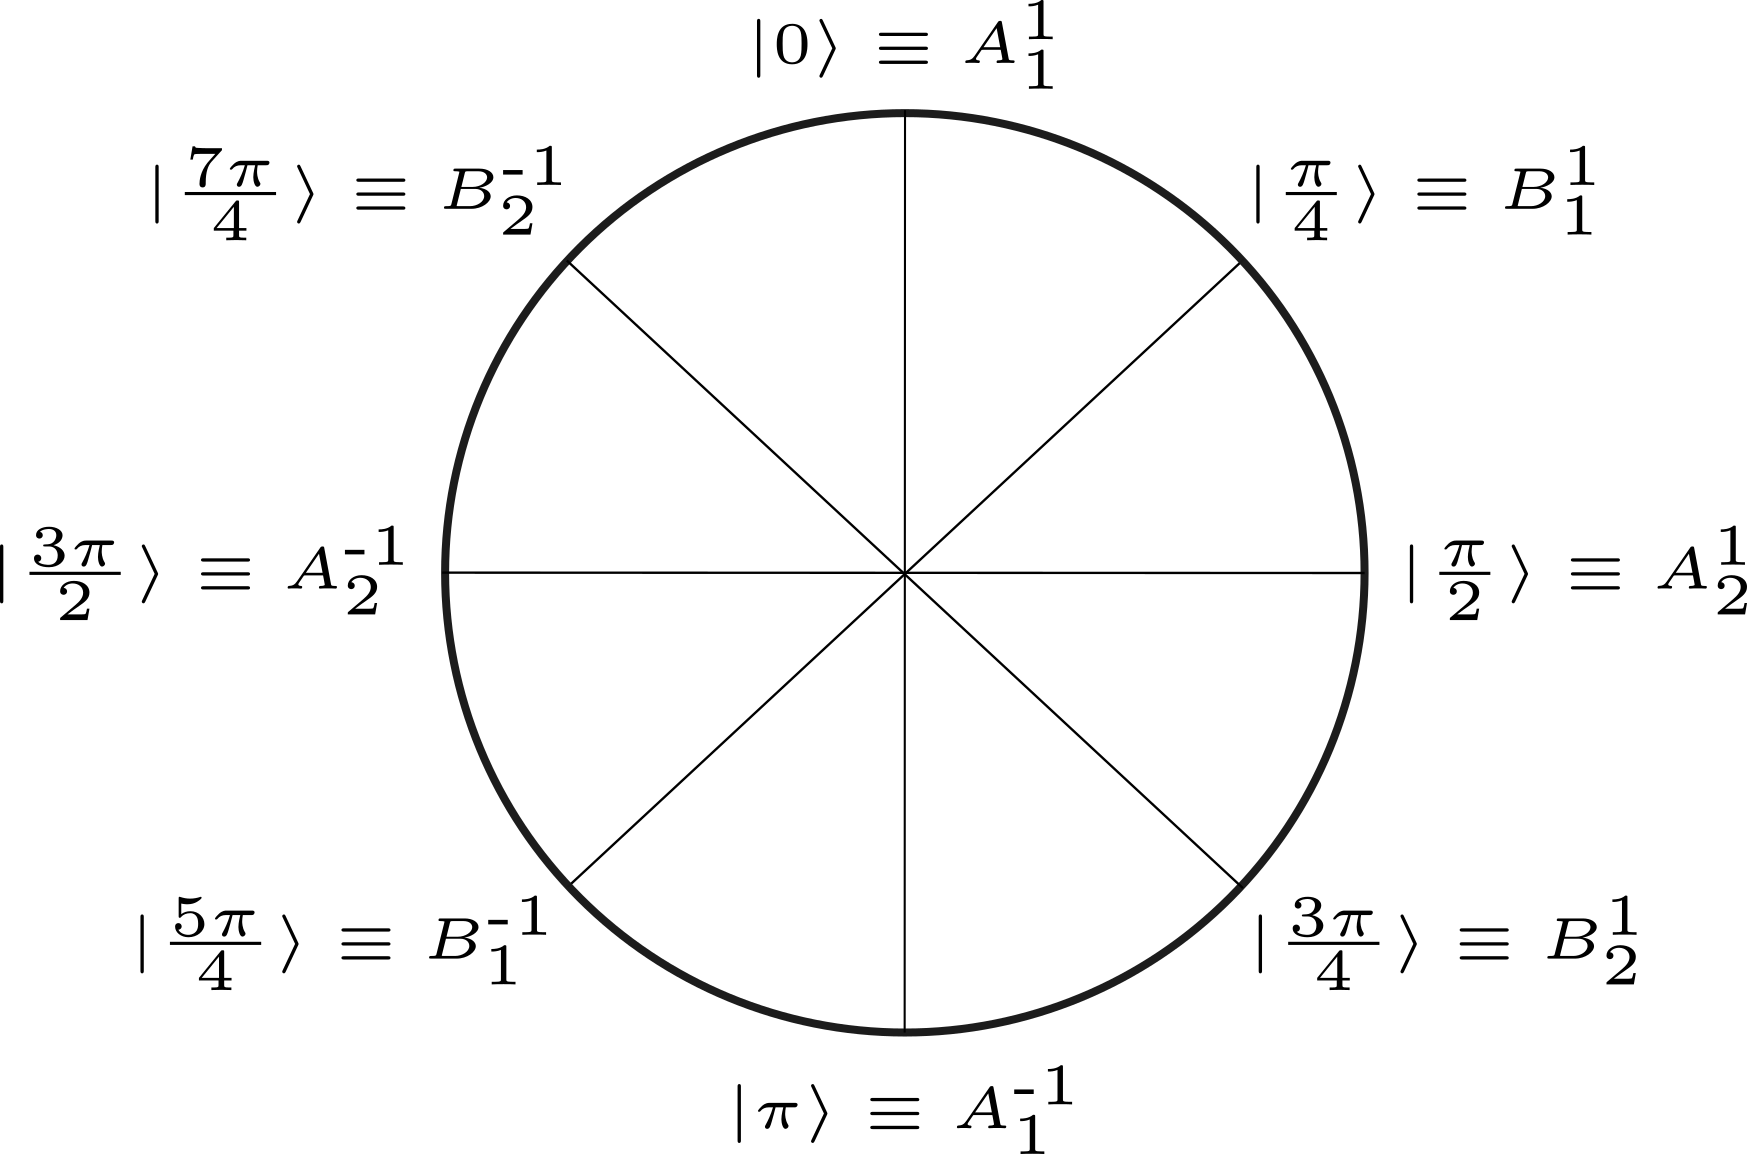
\includegraphics[width=0.5\textwidth]{images/chshmnts.png}
    \caption{The two outcomes of each of the four local projective CHSH measurements $A_1$, $A_2$, $B_1$, and $B_2$ correspond to two antipodal surface points in the xz-plane of the Bloch sphere. For example, the projector associated with the outcome 1 of the measurement $A_1$ projects onto the state $\ket{0}$. The overlap between two states that are related via a rotation by $\frac{\pi}{4}$ in real space have an overlap of $\cos(\frac{\pi}{8})$. By inspection, one sees that the winning CHSH correlations in Figure \ref{fig:chshmnts} are obtained with the probability $\cos^2(\frac{\pi}{8})$.}
    \label{fig:chshmnts}
\end{figure}

In view of Section \ref{sec:self-testing}, important properties of the CHSH Bell test are:
\begin{itemize}
    \item The choice of quantum state and measurements above leads to a maximal violation of the CHSH inequality, as allowed by QM. We will show this in Section $\ref{sec:csw}$. The quantum supremum $B_\mathcal{Q}$ of a Bell inequality's left hand side is called its Tsirelson bound. The Tsirelson bound of the CHSH Bell inequality is $\frac{1}{2}(1+\frac{1}{\sqrt{2}})$.
    \item Assuming projective measurements, all quantum experiments $\expval{\Pi_{A_i}^x\otimes\Pi_{B_j}^y}{\Psi}$ producing a maximal violation of the CHSH Bell inequalitiy are essentially equivalent and related by some trivial operations. This property gives rise to the notion of self-testing and will be discussed in more detail in Section \ref{sec:self-testing}.
\end{itemize}

A generic Bell inequality in the bipartite scenario is of the form
\begin{equation}
\sum_i w_i p(\epsilon_i)\leq B_\mathcal{L}\;,
\label{eqn:bellineq}
\end{equation}
where $w_i>0$ and $\epsilon_i$ denotes the $i$-th measurement event. For now, assuming bipartite Bell tests, a measurement event can be thought of as just an initial preparation $P$ of the system (for instance in an EPR state), followed by both parties performing some local measurement $a$,$b$, and obtaining outcomes $x$,$y$: $a,b \vert x,y$. We have used the same notation as in \cite{Cabello2014} and will revisit the proposed graph-theoretic framework in more detail in Section \ref{sec:csw}, in order to identify the maximal quantum violation of a general KS non-contextuality inequality. Note that all linear combinations of probabilities pertaining to our correlation experiment can be expressed as a positive linear combination with $w_i>0$, like in \ref{eqn:bellineq}. For any negative $w_i$ we may rewrite 
\begin{equation*}
w_i p(e_i)=w_i p(x_i,y_i\vert a_i,b_i)=w_i-w_i\sum\limits_{(x_i',y_i')\neq(x_i,y_i)} p(x_i',y_i' \vert a,b)\;,
\end{equation*} obtaining a positive linear combination of probabilites. 

The statistics of a Bell-type correlation experiment are fully characterized by the set $\{p(x,y\vert a,b)\}_{x,y,a,b}$. For the CHSH experiment, this set contains $2^4=16$ values between 0 and 1, which obey some normalization conditions and can be represented by a vector in $\mathbb{R}^{16-4}=\mathbb{R}^{12}$. Identifying permissible correlations as a subset of $[0,1]^{12}$, in the case of CHSH, one can characterize the geometry of correlations that are compatible with say local causality, quantum theory, or the no-signalling principle. Each set of permissible correlations is clearly convex: While one can check that convex combination preserves the relevant constraints, there is an intuitive argument as to why this must be the case: Assume that we have two experimental procedure, each producing ``allowed" statistics. As we only impose constraints on what correlations we consider to be ``allowed", the actual existence of procedures generating these correlations cannot be discarded. We now consider the following new experimental procedure: we generate a random bit and then perform the ``old" experimental procedure corresponding to the value of the generated bit. By changing the bias of our ``coin", we can produce all statistics that are convex combinations of the initial, permissible statistics.

As discussed, all correlations $p(x,y\vert a,b)$ compatible with an ontological model obeying local causality are convex combinations of local, deterministic probability assignments $p_A(x \vert a,\lambda)p_B(y \vert b,\lambda)$. There are $2^4=16$ distinct such assignments. Thus, the set of local correlations 
\begin{equation*}
\mathcal{L} =\{\{p(x,y\vert a,b)\}_{x,y,a,b}\equiv \vec{v}\in\mathbb{R}^{12}: \vec{v}\; \text{compatible with local causality}\}
\end{equation*}
is a polytope in $\mathbb{R}^{12}$ with 16 extremal vertices. A Bell inequality \ref{eqn:bellineq} defines a separative hyperplane that splits $[0,1]^{12}$ in two, such that $\mathcal{L}$ lies entirely on one side of this hyperplane (the closed half-space). The Bell hyperplane could for instance be a facet of the local polytope, as shown in Figure \ref{fig:correlations}. A facet of $\mathcal{L}$ is one of its delimiting hyperplanes. Bell's Theorem tells us that the set of quantum correlations $\mathcal{Q}$ is strictly larger than $\mathcal{L}$. The set $\mathcal{Q}$ further cannot be characterized in terms of a finite number of delimiting hyperplanes (linear inequalities) \cite{Brunner2014}. Correlations that maximally violate the CHSH Bell inequality have a maximal distance to the Bell hyperplane.

The no-signalling principle is built into the tensor product representation of traditional QM. As such, the set $\mathcal{Q}$ is contained in the set $\mathcal{NS}$, which contains all correlations that obey no-signalling. Like $\mathcal{L}$, $\mathcal{NS}$ is a polytope: $\mathcal{NS}$ is the intersection of $[0,1]^{16}$, the hyperplanes corresponding to normalization constraints $\sum_{x,y} p(x,y\vert a,b)=1$, and those defined by the no-signalling conditions
\begin{align*}
\sum_y p(x,y\vert a,b) & = \sum_y p(x,y\vert a,b') \; \text{and} \\
\sum_x p(x,y\vert a,b) & = \sum_x p(x,y\vert a',b)\;.
\end{align*}
The set $\mathcal{NS}$ is strictly bigger than $\mathcal{Q}$, as there exist correlations, such as the ``PR-box", that satisfy the no-signalling principle and win the ``CHSH game" with certainty \cite{Brunner2014}.

Analogous to Bell inequalities, KS non-contextuality inequalities define hyperplanes that splits the convex set of all permissible correlations in two, such that the closed half-space contains all correlations compatible with a KS non-contextual HVM description.

\begin{figure}
    \centering
    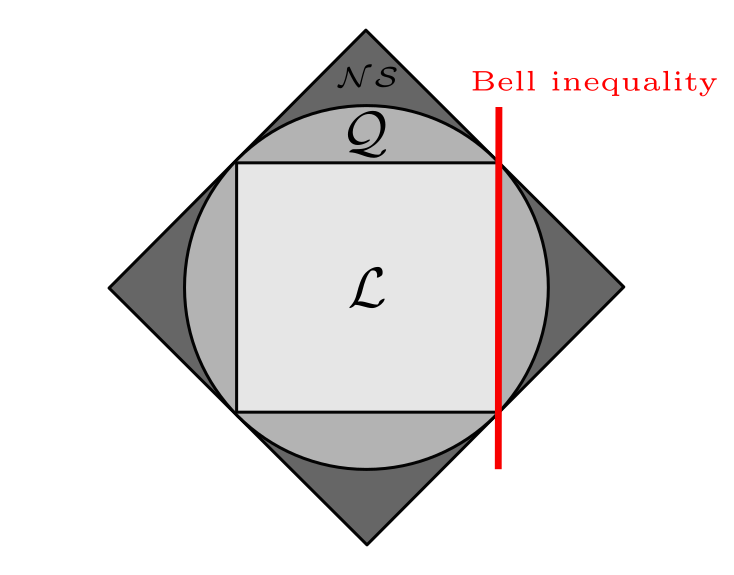
\includegraphics[width=0.5\textwidth]{images/correlations.png}
    \caption{Schematic drawing depicting the geometry of the convex sets $\mathcal{L}$, $\mathcal{Q}$, and $\mathcal{NS}$, containing all local, quantum, and no-signalling correlations, respectively. The sets $\mathcal{L}$, $\mathcal{NS}$ are polytopes and can be characterized by a finite number of facet hyperplanes, whereas the set $\mathcal{Q}$ is more complicated. A Bell inequality, like the CHSH inequality, defines a separative hyperplane such that all local correlations $\mathcal{L}$ lie to one ``side" of this hyperplane.}
    \label{fig:correlations}
\end{figure}

We have captured the essence of Bell's Theorem, cast in a quantum framework, proving that the predictions of QM are incompatible with a local HVM description. Let us now study the relationship between KS non-contextuality and Bell's notion of local causality, or equivalently local determinism (recall Fine's Theorem \cite{Fine1982}). 

The assumption of local determinism is an assumption of context independence for remote measurement contexts, like for Bell-type setting \cite{Spekkens2012}. Both boil down to measurement outcomes being independent of which remote measurement is simultaneously performed (and its outcome). It is important to keep in mind however that KS non-contextuality is a more general assumption, as compatible measurements are not required to be remote.
As Bell's Theorem implies the impossibility of a local HVM of QM, it in particular also proves the impossibility of a KS non-contextual deterministic HVM of QM. This, together with the fact that locality is accepted as a fundamental pillar of modern physics, is why Bell's Theorem is considered to be stronger than the KS Theorem. 

Informally speaking, Bell's Theorem, as presented above, is proof of a KS Theorem in four dimensions, with the nice property that KS non-contextuality is only assumed when it can be justified by locality. A caveat that stems from only assuming KS non-contextuality for remote measurement contexts is that the CHSH proof assumes an entangled state preparation $\ket{\Psi}$. In contrast, the KS Theorem, as formally stated in Theorem \ref{thm:ksthm}, is entirely measurement-dependent. Theorem \ref{thm:ksthm} states that any attempt to assign outcomes to measurements in a KS non-contextual manner is inherently contradictory, no matter the state preparation. In Section \ref{sec:4dim} we examined a KS proof in four dimensions that made use of the full extent of KS non-contextuality. Unsurprisingly, “watering down” the assumption of KS non-contextuality, like in the CHSH proof, requires us to make an additional assumption in order to arrive at a contradiction. For the CHSH proof this assumption is that of a fixed, entangled quantum state. 

Mermin gives a GHZ-like proof of an eight-dimensional KS Theorem \cite{Mermin1993}, which can be recast into a proof of Bell's Theorem, further highlighting the deep connection between both theorems. Again, the information “lost” in assuming KS non-contextuality only when justified by locality is compensated for by a fixed quantum state. Thus, the fact that the KS Theorem is only measurement-dependent and in particular makes no reference to the system preparation is a consequence of the stronger assumption of KS non-contextuality imposed by the KS Theorem.

On a final note, it is worth pointing out that the statement of the KS Theorem is of a fundamentally different nature than that of Bell's Theorem. In particular, it does not propose inequality constraints on correlations that, when found to be violated, would imply the impossibility of a particular classical description. The KS Theorem goes further than that and deduces the impossibility of such an attempt altogether, only by geometric considerations that lead to a contradiction. Nevertheless, this strength is also a key weakness of the theorem. A Bell inequality is operationally testable and does not make reference to the formalism of QM. The general form of correlations compatible with a local HVM description \ref{eqn:lhvm} makes sense, independent of QM. Therefore, the CHSH Bell inequality also holds for theories beyond QM. An experimental observation of a Bell inequality violation implies that there can be no operational theory of reality (compatible with experimental observations) that admits of a locally causal hidden variable theory, quantum theory only being one possible candidate. Any such theory would be in conflict with the experimental data which violates Bell inequalities. By comparison, the KS Theorem is formulated within the framework of QM, for instance making explicit reference to the system's Hilbert space. Therefore, the scope of the KS Theorem is limited to quantum theory. 

In Section \ref{sec:spekkcont} we revise the traditional notion of KS non-contextuality. Spekkens proposes a largely operational notion of non-contextuality that addresses these shortcomings \cite{Spekkens2005}. However, for the purposes of self-testing, which assumes the validity of QM, the main asset of Spekkens contextuality will be that it allows for a consistent treatment of unsharp POVM quantum measurements.

\section[State-dependent KS contextuality\\ The KCBS inequality and odd n-cycle scenarios]{State-dependent KS contextuality \\ \large{The KCBS inequality and odd n-cycle scenarios}}
\label{sec:kcbs}
In Section \ref{sec:formalproof} we found that for every projective Hilbert space of dimension $\geq$ 3 there exists a finite set of rays for which there exists no KS non-contextual value assignment according to Definition \ref{def:kscontbasis}. Identifying these rays with projective measurements of rank one gives us a set of projective measurements for which there exists no KS non-contextual value assignment according to Definition \ref{def:kscontherm}. We call such sets of projective measurements (or rays in a projective Hilbert space) KS uncolourable, owing to the fact that one can reduce the problem of finding a valid KS non-contextual value assignment to a colouring problem, as was done in Section \ref{sec:formalproof}. 
\begin{definition}
A set of projective measurements (rays in a projective Hilbert space) is called \emph{KS colourable} if there exists a KS non-contextual assignment of measurement outcomes (values 0,1) to the measurements (rays) in the set. If there exists no such value assignment, the set is called \emph{KS uncolourable}.
\end{definition}
KS uncolourable sets embody the ``strongest" proofs that QM is incompatible with a KS non-contextual HVM description, in the sense that the structure in the set of measurements alone is enough to arrive at a logical contradiction.
Nevertheless, as alluded to in Section \ref{sec:bell}, also KS colourable sets of projective measurements may exhibit KS contextuality. This manifests itself in QM predicting violations of KS non-contextuality inequalities for some KS colourable sets. A KS non-contextuality inequality is, analogously to a Bell inequality, a linear inequality constraint on the convex set of correlations that is satisfied for all correlations compatible with a KS non-contextual HVM description. We will discuss the simplest KS non-contextuality inequality, the KCBS inequality, as well as an infinite class of generalizations thereof. These KS non-contextuality inequalities allow for self-testing, as will be the subject of Section \ref{sec:contselftesting}. Before that, note that we have already come across one example of a KS non-contextuality inequality, the CHSH inequality, albeit in the context of Bell nonlocality. The set of CHSH measurements given in Section \ref{sec:bell} that produce a maximal violation of the CHSH inequality when acting on an EPR pair is a KS colourable set of projective measurements. QM predicts state-dependent Bell non-locality, as witnessed by violations of the CHSH inequality. For reasons highlighted in Section \ref{sec:bell}, the CHSH inequality is also a KS non-contextuality inequality and the non-local correlations of the CHSH experiment exhibit state-dependent KS contextuality. Programming the source to emit separable bipartite states, as opposed to EPR pairs, will yield KS non-contextual correlations.

Note that there even exist KS colourable sets of measurements that produce state-independent KS contextuality, in the sense that QM predicts the violation of a KS non-contextuality inequality for all possible quantum state preparations. An example of such a set is one proposed by Yu and Oh \cite{Yu2012}, simply called the Yu-Oh set. It is a set of 13 rank one projectors that act on a three-dimensional Hilbert space. In fact, if one identifies the rank one projectors with rays in a projective Hilbert space, the 13 Yu-Oh rays are a subset of the 33 rays of the Peres configuration that we used in proving the KS Theorem in Section \ref{sec:formalproof}. The Yu-Oh set is the minimal set of rays revealing state-independent KS contextuality, as proved in \cite{Cabello2016a}.

The perhaps simplest example of a quantum experiment leading to (state-dependent) KS contextuality for a single quantum system is the KCBS scenario \cite{Klyachko2008}. We will present the corresponding KCBS KS non-contextuality inequality, which will become relevant when we later discuss self-testing of quantum systems in Sections \ref{sec:self-testing} and \ref{sec:contselftesting}. 

For the KCBS KS contextuality scenario we assume five dichotomic projective measurements with outcomes 0 and 1. Additionally, the five measurements should obey cyclic compatibility, as shown in Figure \ref{fig:kcbscompat}. We freely choose a pair of compatible measurements (measurement context) at random, each with equal probability, and determine the value of the following linear sum of probabilities:
\begin{equation*}
    \sum_{i=1}^5 p(0,1\vert i, i+1)\leq 2,
\end{equation*}
where compatibility with a KS non-contextual HVM imposes an upper bound of 2 for this expression: For any HVM description of the KCBS experiment, $\sum_{i=1}^5 p(0,1\vert i,i+1)$ can be rewritten as $\int_{\Lambda}d\lambda\thinspace\mu(\lambda\vert i,i+1)\sum_{i=1}^5 p(0,1\vert i, i+1, \lambda)$, where $\mu$ is some probability density function over the ontic state space $\Lambda$. Furthermore, $\mu(\lambda\vert i,i+1)=\mu(\lambda)$, as we assume the choice of measurement context to be uncorrelated with the system. Analogously to Specker's three boxes or the CHSH experiment, one can easily verify that this quantity has a non-trivial upper bound for any KS non-contextual HVM description.

\begin{figure}
    \centering
    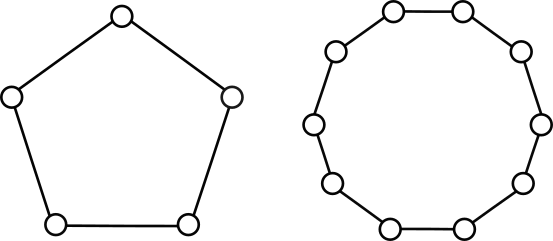
\includegraphics[width=0.6\textwidth]{images/kcbscompat.png}
    \caption{Graph showing compatibility relations for the KCBS (left) and a higher order odd $n$-cycle scenario (right). Each vertex corresponds to one projective measurement, adjacent measurements are compatible.}
    \label{fig:kcbscompat}
\end{figure}

We now present a quantum experiment involving a KS colourable set of five projective measurements on a qutrit for which QM predicts a (maximal) violation of the KCBS KS non-contextuality inequality. The five projective measurements of this reference experiment correspond to five rank one projectors that project onto five pure qutrit states. The components of these five qutrit states with respect to the standard qutrit basis $\{\ket{0}, \ket{1}, \ket{2}\}$ are real, allowing us to represent them as vectors in $\mathbb{R}^3$, see Figure \ref{fig:kcbsref}. The angle between each of the five vectors and the $\vert 0\rangle$ qutrit axis is $\cos^2(\theta)=\frac{1}{\sqrt{5}}$. The following is an explicit expression for five suitable qutrit states that also satisfy cyclic compatibility:
\begin{align*}
    \ket{u_j} = \left(\cos(\theta),\thinspace\sin(\theta)\sin(j\phi),\thinspace\sin(\theta)\cos(j\phi)\right)^T,
\end{align*}
for $\displaystyle j=1\dots 5$ with $\displaystyle\phi=\frac{4\pi}{5}$.

For these five projective measurements acting on the $\vert 0\rangle$ qutrit state, QM predicts \begin{equation*}
\sum_{i=1}^5p(0,1\vert i, i+1)=\frac{5}{\sqrt{5}}=\sqrt{5}>2.    
\end{equation*}
Not only does the reference quantum experiment $\ket{0}$, $\{\ket{u_i}\}_{i=1}^5$ produce correlations that violate the KCBS non-contextuality inequality, but this violation is also maximal, as we will see in Section \ref{sec:csw}.

\begin{figure}
    \centering
    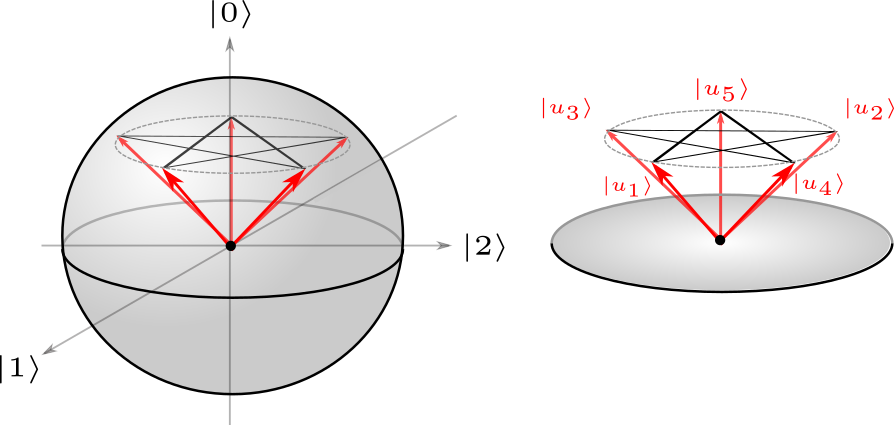
\includegraphics[width=0.9\textwidth]{images/kcbsref.png}
    \caption{Reference KCBS experiment on a qutrit leading to a maximal violation of the KCBS KS non-contextuality inequality. An experimenter can freely choose between five rank one projective measurements $\ket{u_i}$ that satisfy cyclic compatibility: $\bra{u_i}\ket{ u_{i\oplus1}} = 0$. The qutrit is initially prepared in the state $\ket{0\rangle}$ and then measured in one of five measurement contexts (i,i$\oplus$1). After the measurement the qutrit state is reset.}
    \label{fig:kcbsref}
\end{figure}

One can generalize the KCBS KS non-contextuality inequality to greater cycle lengths $n$. For the odd integers $n\geq 5$, where $n$ parametrizes the number of dichotomic projective measurements obeying cyclic compatibility, one finds a class of KS non-contextuality inequalities \cite{Bharti2019}
\begin{equation}
    \label{eqn:oddncycleclass}
    \sum_{i=1}^n p(0,1\vert i,i+1) \leq \frac{n-1}{2}.
\end{equation}
The quantum supremum for a given cycle length $n$ is
\begin{equation}
\label{eqn:ncyclequsup}
B_q^{(n)}=\frac{n\cos(\frac{\pi}{n})}{1+\cos(\frac{\pi}{n})}\,,
\end{equation} and can be achieved by preparing the qutrit state $\ket{0}$ and performing the rank one projective measurements
\begin{equation}
\label{eqn:ncycleideal}
\vert u_j^{(n)}\rangle = \left(\cos(\theta_n),\thinspace\sin(\theta_n)\sin(j\phi_n),\thinspace\sin(\theta_n)\cos(j\phi_n)\right)^T,
\end{equation}
for $j=1\dots n$, $\displaystyle\cos^2(\theta_n)=\frac{\cos(\frac{\pi}{n})}{1+\cos(\frac{\pi}{n})}$, and $\displaystyle\phi=\frac{(n-1)}{n}\pi$.

In Section \ref{sec:csw}, we adopt the graph-theoretic framework proposed in \cite{Cabello2014} to classify correlations of an arbitrary experiment. It turns out that for a general linear combination of probabilities one can relate the KS non-contextual and quantum suprema to certain graph invariants. Computing these graph invariants corresponds to solving a mathematical optimization problem. In view of self-testing, this will enable us to identify extremal correlations and study whether these can only be realized in an essentially unique manner.